\documentclass[output=paper]{langscibook}
\title{The negative existential cycle in Bantu}
\author{%
Rasmus Bernander\affiliation{University of Helsinki} and
Maud Devos\affiliation{Ghent University} and
Hannah Gibson\affiliation{University of Essex}%
}
% \chapterDOI{} %will be filled in at production

%\epigram{Change epigram in chapters/01.tex or remove it there }
%Ljuba made changes in the file Bantu-Bernander-Devos-Gibson.tex on April 18, 2021. Do not use this version.

\abstract{Renewal of negation has received ample study in Bantu languages. Still, the relevant literature does not mention a cross-linguistically recurrent source of standard negation, i.e., the existential negator. The present paper aims to find out whether this gap in the literature is indicative of the absence of the Negative Existential Cycle (NEC) in Bantu languages. It presents a first account of the expression of negative existence in a geographically diverse sample of 93 Bantu languages. Bantu negative existential constructions are shown to display a high degree of formal variation both within dedicated and non-dedicated constructions. Although such variation is indicative of change, existential negators do not tend to induce changes at the same level as standard negation. The only clear cases of the spread of an existential negator to the domain of standard negation in this study appear to be prompted by sustained language contact.

\textbf{Keywords:} Bantu languages, negation, language change, morphology
}

\maketitle
\begin{document}

\section{Introduction}\label{sec:1:1} The Bantu\il{Bantu|(} language family
comprises some 350--500 languages spoken across much of Central, Eastern
and Southern Africa. According to \citet{Grollemund2015}, these languages
originate from a proto-variety of Bantu, estimated to have been spoken
roughly 5000 years ago in the eastern parts of present-day northwest
Cameroon. Many Bantu languages exhibit a dominant SVO word order. They are
primarily head-marking, have a highly agglutinative morphology and a rich
verbal complex in which inflectional and derivational affixes join to an
obligatory verb stem. The Bantu languages are also characterised by a
system of noun classes -- a form of grammatical gender. By convention,
these classes are numbered with odd and even pairings commonly representing
singular and plural forms. Many Bantu languages also have locative classes
containing only  locative nouns. The most widespread locative classes are
referred to as 16, 17 and 18 and are marked by *{\it pa-}, *{\it kʊ-} and
*{\it mʊ-} respectively. These prefixes have been reconstructed for
Proto-Bantu and refer to
specific, general and internal location.\footnote{Other less prevalent
strategies for locative noun formation include the use of the class 23/25
locative prefix *{\it ɩ-} (cf.
\citealt{Gregoire1975,Maho1999})\ia{Gr\'egoire, Claire}\ia{Maho, Jouni} and
the locative suffix {\it -(i)ni} \citep{SamsonSchadeberg1994}.\ia{Samson,
Ridder}\ia{Schadeberg, Thilo C.}} The locative noun classes will be central
to the discussion in this paper, as they are ubiquitous in the formation of
both affirmative and negative existentials in Bantu, as will become clear
further below.

The Bantu languages exhibit a high degree of variation in the encoding of
negation within the clause. However, some recurrent patterns can be
observed. Negation most commonly involves verbal affixes, typically either
a pre-initial marker (appearing before the subject prefix) or a
post-initial marker (following the subject prefix). The former tends to be
reserved for negation in declarative main clauses (i.e. standard negation),
whereas the latter is commonly used for negation in non-standard clause
types such as infinitive, subjunctive, imperative, relative and dependent
clauses. Examples of pre-initial and post-initial negative strategies are
given in \REF{ex:swahili-read} and \REF{ex:swahili-go},
respectively.\footnote{The classification of the Bantu languages in this
paper is based on \citet{Maho2009},\ia{Maho, Jouni} which is an updated
version of \citegen{Guthrie1971}\ia{Guthrie, Malcolm} classification, in
which languages are divided into geographic zones which are assigned
letters. These groupings are in turn divided into smaller groups indicated
by the decimal digits. The final digit represents a specific language
within such a group. Letters and additional digits after this digit refer
to varieties of the same language. The ISO-codes of the languages of the
sample are given in \tabref{tab:1:1} the Appendix. Languages which are
discussed but are not part of the sample have their ISO-code in the running
text.} As can be seen in \REF{ex:swahili-problem}, \ili{Swahili} uses the
standard negative marker {\it ha-} in negative existential clauses.
\ea\label{ex:swahili-read-go-problem} \langinfo{Swahili}{}{G42}\\
\ea\label{ex:swahili-read} 
\gll ha-tu-ta-som-a ki-tabu hiki\\ 
{\sc neg-sm}1pl-{\sc fut}-read-{\sc fv} 7-book 7.{\sc dem}\\ 
\glt `We will not read this book.'\\ 
\ex\label{ex:swahili-go} 
\gll u-si-end-e\\ 
{\sc sm2}sg-\textsc{neg}-go-{\sc sbjv}\\ 
\glt `Do not go!' 
\ex\label{ex:swahili-problem}
\gll ha-ku-na ma-tata\\ 
{\sc neg-sm17-com} 6-problem\\ 
\glt `There are no problems.' \z\z

Other recurrent negation strategies involve pre-verbal and post-verbal
enclitics/particles, and periphrastic constructions employing an inherently
negative auxiliary and an infinitive. Negative stacking -- the combination
of different negation strategies for the expression of negation -- is also
attested. Such variation is indicative of change. Although renewal of
negation in Bantu has received ample attention in previous studies (e.g.
\citealt{KambaMuzenga1981,Guldemann1996,Guldemann1999,DevosAuwera2013,DevosOlmen2013}),\ia{Kamba
Muzenga, J. G.}\ia{G{ü}ldemann, Tom}\ia{Devos, Maud}\ia{Van der Auwera,
Johan}\ia{Van Olmen, Dani{ë}l} there has been no systematic study of the
form and variation of negative existential constructions, nor of changes
indicative of a negative existential cycle
\parencites{Croft1991}{Veselinova2016}.\ia{Croft,
William}\ia{Veselinova, Ljuba} This paper seeks
to address this gap in the literature through an examination of negative
existentials across a sample of 93 Bantu languages, as listed (along with
their ISO-codes) in \tabref{tab:1:1} in the Appendix. The aim is to provide
the first exploration of negative existentials in Bantu languages, as well
as to examine the extent to which the stages of the negative existential
cycle, as set out by \citet{Croft1991}\ia{Croft, William} and
\citet{Veselinova2016},\ia{Veselinova, Ljuba} can be identified in the
language family.\footnote{It should be noted that the depth of our analysis
naturally depends on the descriptive status of the languages under
examination.}

The paper is structured as follows: In \sectref{sec:1:2},
 we examine the renewal of negative strategies across the Bantu languages.
 In \sectref{sec:1:3}, we present an overview of affirmative existential
 constructions in Bantu, looking at both dedicated and non-dedicated
 strategies for forming existentials. In \sectref{sec:1:4}, we look at the
 distribution of the stages of the negative existential cycle across the
 Bantu sample. In \sectref{sec:1:5}, we chart the development from
 non-dedicated negative existentials to dedicated negative existentials. In
 \sectref{sec:1:6}, we explore additional processes of change. We first
 look at usage extensions beyond verbal negation (\sectref{sec:1:6.1}) and
 towards non-standard negation types (\sectref{sec:1:6.2}). We then discuss the possible involvement of existential negators in instantiations of the Jespersen Cycle (\sectref{sec:1:6.3}) and a specific development attested in varieties of the East African Bantu language \ili{Swahili} (\sectref{sec:1:6.4}). \sectref{sec:1:7} consists of a summary and draws a number of conclusions.

\section{The renewal of negation in Bantu}\label{sec:1:2} In this section
we discuss three recurrent pathways of change in the expression of negation
in Bantu languages. The first two concern the genesis and renewal of the
two main Bantu negation strategies, i.e., the pre-initial and the
post-initial negation strategy. \citet{Guldemann1996,Guldemann1999}
identifies the origin of the former in the merger between an illocutionary
particle (mostly commonly a negative copula) and a (dependent) finite verb
form. He finds evidence for this pathway, {\it inter alia}, in the
recurrent formal similarity between negative copulas and pre-initial
negative markers, as is the case in Nyanja.\il{Chewa\slash Nyanja}\il{Nyanja}
\ea\label{ex:nyanja-go-tuesday} 
%\langinfo{Nyanja}{}{N31a, \citealt[174]{StevickHollander1965}, cited from \citealt[568]{Guldemann1999}} 
\ili{Nyanja}\il{Chewa\slash Nyanja} (N31a, \citealt[174]{StevickHollander1965}, cited from \citealt[568]{Guldemann1999})
\ea\label{ex:nyanja-go} \gll
si-ti-dza-pit-a\\ {\sc neg-sm}1pl-{\sc fut}-go-{\sc fv}\\ \glt `We won't
go.'\\ \ex\label{ex:nyanja-tuesday} \gll lelo si laciwili\\ today {\sc
neg.cop} Tuesday\\ \glt `Today is not Tuesday.’ \z\z Still following
\citet{Guldemann1996,Guldemann1999}, the post-initial strategy is assumed
to have its origin in a periphrastic construction consisting of an
inherently negative auxiliary followed by an infinitive. Evidence for this
second pathway comes from the functional overlap between these
constructions in different present-day languages. Both post-initial
negation and periphrastic negation involving a negative auxiliary are
typically used for the negation of marked clauses, i.e., to negate
infinitives, subjunctives, imperatives, relatives and dependent clauses.
Compare the use of the post-initial strategy in example \REF{ex:swahili-go}
from \ili{Swahili} with the use of the periphrastic strategy for prohibition in
Manda\il{Manda} shown in \REF{ex:manda-fish}.  \ea\label{ex:manda-fish}
\langinfo{Manda}{}{N11, \citealt[664]{Bernander2018}}\\ \gll Ø-kótúk-áyi
ku-túmbúl-a ku-lóv-a sómba\\ Ø-{\sc neg-ipfv.sbjv} 15-begin-{\sc inf}
15-fish-{\sc inf} 10.fish\\ \glt `Don't begin to fish.' \z
\citet{Bernander2017,Bernander2018} offers a language-internal
instantiation of this pathway. In Manda, the cessative auxiliary
\textit{-kotok-} `leave (off), stop’\footnote{Note that \textit{-kotok-}
becomes \textit{-kotuk-} before the imperfective suffix, cf.
\REF{ex:manda-fish}.} has spread from indicating prohibition to indicating
the other marked negation types identified by
\citet{Guldemann1996,Guldemann1999}, with the exception of negative
relatives. The Manda\il{Manda} data also further add weight to
\citegen[191]{Nurse2008} claim that prohibitives are ``a major conduit
through which innovation occurs''. At first, the prohibitive marker spreads
to other more marked negation types, as seen in Manda. However, if
\citegen[193, fn 25]{Nurse2008} suggestion that several post-initial
negative markers in northwestern Bantu languages of zones A and C are
derived from the cessative auxiliary *\textit{d{\`e}k} `let, let go, cease,
allow' \citep{BastinCoupez2002} holds true, further spread to standard
negation may also be attested. In Nugunu,\il{Nugunu} for example, the
post-initial negative marker \textit{-de-} is used for all negation types,
i.e., for negation of both marked clauses and standard clauses
\citep{Nurse2007}. Examples \REF{ex:nugunu-beat} and \REF{ex:nugunu-give}
show the use of \textit{-de-} for prohibition and standard
negation.\footnote{Note that \textit{-de-} becomes \textit{-dɔ-} after [ɔ]
in Nugunu.\il{Nugunu}} 
\ea\label{ex:nugunu-beat-give}
\langinfo{Nugunu}{}{A62, \citealt{Nurse2007}} \ea\label{ex:nugunu-beat}
\gll ɔ-dɔ-g{\'ɔ}ba\\ {\sc sm}2sg-{\sc neg}-beat\\ 
\glt `do not beat'\\
\ex\label{ex:nugunu-give} \gll a-de-mb{\'a}-f{\^a}\\ {\sc sm}1-{\sc
neg-pfv}-give\\ 
\glt `s/he hasn't given' \z\z 
%
The third pathway of change
concerns recurrent instances of double negation in Bantu languages, i.e.,
the combination of the (inherited) pre-initial or post-initial negative
marker and a post-verbal negative marker in a single negative strategy, as
illustrated in (5) from Ruwund.\il{Ruwund} \ea\label{ex:ruwund:l53}
\langinfo{Ruwund}{}{L53, \citealt[696]{Nash1992}}\\ \gll
k{\`e}-z-in-{\`a}-p\\ {\sc neg.sm}1-come-{\sc prs.cont-fv-neg}\\ \glt `S/he
is not coming.' \z Double negative marking is suggestive of a Jespersen
Cycle, a process whereby an additional negator is first used to reinforce
negation, then becomes an obligatory part of negation and eventually ends
up as the only exponent of negation. This final stage, with only a single
negator, is illustrated with the Manda\il{Manda} example in
\REF{ex:manda-security}.  
\ea\label{ex:manda-security}
\langinfo{Manda}{}{N11, \citealt[308]{Bernander2017}}\\ 
\gll ni-ng'-g{\'a}n-a l{\'e}pa {{\'o}f{\'\i}sa wa usal{\'a}ma}\\
\textsc{sm1}sg-\textsc{om}1-like-\textsc{fv} \textsc{neg} {security
officer}\\ \glt `I do not like the security officer.' \z
\citet{DevosAuwera2013} show that the Jespersen Cycles can indeed be
observed in Bantu languages. This observation follows the lead of several
Bantu grammarians, as well as \citet[256--258]{Guldemann1996},
\citet[7]{GuldemannHagemeijer2006}, \citet[165]{Guldemann2008},
\citet[57]{Nurse2008}, and \citet[117]{Guldemann2011}, who link double
negation in Bantu to its most famous example in French \textit{ne \ldots{}
pas}. \citet{DevosAuwera2013} identify several sources of post-verbal
negative markers and show that the post-verbal negative marker may become
the only exponent of negation but that a Jespersen Cycle might also set in
at this doubling stage, resulting in triple or even quadruple negation (for
an example of the latter see \citealt{DevosTshibanda2010}). Triple negation
in Salampasu\il{Salampasu} [slx] is shown in
\REF{ex:salampasu-cut}.
\ea\label{ex:salampasu-cut} \langinfo{Salampasu}{}{L51,
\citealt{Ngalamulume1977}, cited from \citealt[210]{DevosAuwera2013}}\\
\gll k{\'a}{\'a}-d{\'e}d{\'e}ki-k{\'u} ny-t{\'o}nd{\'u}  ba\\
\textsc{neg.sp}1-cut.\textsc{pfv-neg} 3-tree \textsc{neg}\\ \glt `He has
not cut a tree.' \z 

\section{Existential constructions in Bantu}\label{sec:1:3} 
As will become apparent in \sectref{sec:1:4} and
\sectref{sec:1:5}, a significant number of Bantu languages express
negative existence merely through (standard) negation of the affirmative
existential construction. This fact merits a brief presentation of the
versatile tactics for forming affirmative existentials found across Bantu,
before embarking on the main topic, i.e., their negative counterparts. The
results presented in this section are based on \citet{BernanderDevos2018},
an investigation into the expression of affirmative existentials across
Bantu, departing from a definition of such expressions in relation to plain
locational clauses. In line with \citet{Creissels2014,Creissels2015},
existentials are conceptualized as providing an alternative way of encoding
the prototypical figure-ground relationship of a plain locational. That is,
in existentials, the ground rather than the figure is the perspectival
center. Several different tactics for expressing existence have been found
in different languages, but also within a single language variety. Of
these, an initial division can be made between those expressions of
existential predication which, except for word order changes, are not
different from locational clauses (\sectref{sec:1:3.1}) and those
constructions that are dedicated to the expression of existential
predication (\sectref{sec:1:3.2}).

\subsection{Non-dedicated existentials}\label{sec:1:3.1}
In roughly 20\% of the cross-Bantu sample, existential predication was found to be formally identical to locational existential predication \citep{BernanderDevos2018}. However, although there are no morphosyntactic differences between a plain locational construction and existential predication in these cases, it should be noted that the existentials are recurrently pragmatically marked. Typically, there is a shift to presentational word order, where the (logical) subject ends up in post-verbal position. This tendency is also pervasive in both dedicated existential constructions and negative existentials and it adheres to a wider cross-linguistic tendency (see e.g. \citealt{Freeze1992,BentleyCiconte2013}).\footnote{In fact, the only examples of languages which do not exhibit such a permutation are spoken in the very north-western part of the Bantu speaking region. These languages are therefore in close or direct contact with the ``Macro-Sudan belt'' \citep{Guldemann2008}. The Macro-Sudan belt is a linguistic area characterized as being ``devoid of dedicated existential predicative constructions, and with rigid constituent order in locational clauses'' \citep[22]{Creissels2014}.} Example \REF{ex:makhuwa-man} is an instance of an existential marker in \ili{Makhuwa} which is formally under-specified in relation to the plain locational in \REF{ex:makhuwa-table}.
\ea\label{ex:makhuwa-man-table}
\langinfo{Makhuwa}{}{P31, \citealt[109]{Wal2009}}
\ea\label{ex:makhuwa-man}
\gll aa-r{\'\i} nlopwana  m-mots{\'a}\\
     \textsc{sm}1.\textsc{pst}-be 1.man 1-one\\
\glt `There was a man.'\\
\ex\label{ex:makhuwa-table}
\gll eli{\'\i}v{\'u}r{\'u} e-r{\'\i} wa-me{\'e}tsa\\
	9.book \textsc{sm}9-be 16-table\\
\glt `The book is on the table.'
\z\z
Both instances of predication contain the same copula indexed with the
relevant regular subject agreement. The only difference between the two
expressions is the word order permutation of the existential proposition in
\REF{ex:makhuwa-man}, relative to the canonical SVO order of the language,
as found in \REF{ex:makhuwa-table}. Another example comes from
(Standard)\il{Swahili!Standard Swahili}
\ili{Swahili}, where it is once again only the word order which
distinguishes the existential predication of \REF{ex:swahili-agriculture}
from the plain locational predication in \REF{ex:swahili-table}.
\ea\label{ex:swahili-agriculture-table}
\langinfo{Swahili}{}{G42, \citealt[46]{Marten2013}}
\ea\label{ex:swahili-agriculture}
\gll zi-po n-chi amba-zo hu-tegeme-a ki-limo\\
     \textsc{sm}10-\textsc{loc.cop}16 10-country \textsc{rel-refcd}10 \textsc{hab}-depend-\textsc{fv} 7-farming\\
\glt `There are countries which depend on agriculture.'\\
\ex\label{ex:swahili-table}
\gll ki-tabu ki-po meza=ni\\
	7-book \textsc{sm7-loc.cop16} 6.table=\textsc{loc}\\
\glt `The book is on the table.'
\z\z
It should be noted that the existential predication exemplified in
\REF{ex:swahili-agriculture} represents only one of two possible tactics
for the formation of existentials in (Standard) \ili{Swahili}\il{Swahili!Standard
Swahili}, the other tactic being the comitative-existential type which was exemplified in \REF{ex:swahili-problem} in \sectref{sec:1:1} and which is further discussed in \sectref{sec:1:3.2} below. This situation in Swahili reflects a wider tendency of non-dedicated existential predications to alternate with a dedicated existential construction in a single language. 

\subsection{Dedicated existentials}\label{sec:1:3.2}
80\% of the languages in our current dataset use dedicated existentials. Two of Creissels' (\citeyear{Creissels2014,Creissels2015}) seven types of existential predication are frequently and widely attested, namely the ``locative-existential'' type and the ``comitative-existential'' type \citep{BernanderDevos2018}.

The locative-existential type is characterized by the presence of a
locative element which is absent from the plain locational clause.
Locative-existential constructions exhibit differing degrees of
specialization and semantic bleaching of this locative element, but its
locative origin is commonly transparent. Typically, the locative element
stems from what was originally a locative-referential enclitic which
attached to a copula verb and in certain contexts became reinterpreted as
marking existential predication. Another common locative-existential type comprises constructions where the subject marker of the predicator has shifted from referring to the (logical) subject to taking agreement from a locative noun class. Both of these subcategories of locative-existentials can be illustrated by \ili{Cuwabo}, which makes equal use of the two categories. Thus, in example \REF{ex:cuwabo-girl}, the existential is formed with the copula verb \textit{-kala} and an enclitic from the locative class 17, the subject marker of the verb agreeing with the post-verbal (logical) subject. In example \REF{ex:cuwabo-flower}, however, there is no enclitic (although the copula verb is the same). Instead, the existential construction is formed with the locative class 17 as a subject marker.
\ea\label{ex:cuwabo-girl-flower}
\langinfo{Cuwabo}{}{P34, \citealt[465, 466]{Guerois2015}}
\ea\label{ex:cuwabo-girl}
\gll ns{\'a}k\'a ni-modh\'a o-{\'a}-k{\'a}la=wo mw{\'a}n{\'a}-mw{\'\i}yan\'a\\
	5.time 5-one \textsc{sm}1-\textsc{pst.ipfv.cj}-be-\textsc{loc}17 1.child-1.woman\\
\glt `One day, there was a girl.'
\ex\label{ex:cuwabo-flower}
\gll o-tt{\'o}l{\'o}=ni {\'o}k{\'u}l\'e o-hi-ik{\'a}l\'a f{\'u}l{\'o}{\'o}ri\\
	17-well=\textsc{loc} \textsc{dem} \textsc{sm}17-\textsc{pfv.dj}-be   9a.flower\\
\glt `There at the well there is a flower \ldots{}'
\z\z
In a small set of Bantu languages, the existential construction consists of the combination of these two subtypes, as in the example from \ili{Lusoga} in \REF{ex:lusoga-livingroom} where the copula verb is inflected with both a subject marker and an enclitic from the locative noun class 18.
\ea\label{ex:lusoga-livingroom}\il{Lusoga}
\langinfo{Lusoga}{}{JE16, Nabirye p.c. 2016}\\
\gll mu i-d{\'\i}ilo mu-l{\'\i}-mu eb{\'\i}-samp\'a\\
	18 5-living.room \textsc{sm}18-be=\textsc{loc}18 8-mat\\
\glt `In the living room there are mats.'
\z
In some languages, univerbation of a locative element and a copula or light
verb has given rise to two types of `locative/existential predicates'. A first type involves univerbation of a copula or light verb and a locative enclitic. The \ili{Makhuwa} predicate \textit{-h{\'a}avo} in \REF{ex:makhuwa-animal} can reasonably be thought to derive from the light verb \textit{-hala} `stay, remain' to which the class 16 locative enclitic \textit{=vo} is added. Locative post-finals are not (or no longer) productively used in Makhuwa and \textit{-h{\'a}avo} never occurs without the locative enclitic.
\ea\label{ex:makhuwa-animal}
\langinfo{Makhuwa}{}{P31, \citealt[109]{Wal2009}}\\
\gll y-a{\'a}-h{\'a}avo e-n{\'a}m{\'a} e-mots{\'a}\\
	\textsc{sm9-pst}-be.present 9-animal 9-one\\
\glt `There was an animal \ldots{}'
\z
A second type involves univerbation of an erstwhile locative object prefix and a copula. As suggested in \citet{BernanderDevos2018}, the Mawiha\il{Mawiha} predicate \textit{-pawa} in \REF{ex:mawiha-house} has its origin in merger of the class 16 locative object prefix \textit{-pa-} with the copula \textit{-wa} `be'. The (near-) absence of locative object prefixes as obligatory locative elements in Bantu existential constructions of the locative-existential type is probably due to the limited distribution of locative object prefixes in Bantu languages more generally \citep{Marlo2015,ZellerXXXX}.
\ea\label{ex:mawiha-house}
\langinfo{Mawiha}{}{P25, \citealt[105]{Harries1940}}\\
\gll mu-ɲande mwake mu-ndi-pawa {\^w}a-nu\\
	18-9.house 18.\textsc{poss}1 \textsc{sm}18-\textsc{pfv}-be.present 2-people\\
\glt `There are people in his house.'
\z

The second of the two major types of dedicated existential constructions found across the language family is the comitative-existential type. In such a construction, the figure is encoded in a way that is similar to the phrase representing the companion in comitative predication. As illustrated with the example from \ili{Digo} in \REF{ex:digo-man}, Bantu comitative-existential constructions are typically marked with a reflex of the Proto-Bantu reconstructed conjunction/preposition *\textit{na} `and/with' \citep{BastinCoupez2002}.
\ea\label{ex:digo-man}\il{Digo}
\langinfo{Digo}{}{E73, \citealt[320]{Nicolle2013}}\\
\gll hipho kare ku-a-kala na mu-tu m-mwenga\\
  long ago \textsc{sm17-pst}-be with 1.person 1-man\\
\glt `Long ago, there was a man.'
\z
As pointed out by \citet{Creissels2014}, this type of existential
construction is characteristic for the Bantu language family, the extension
of a comitative marker to an existential being rare from a cross-linguistic
perspective. Note that a locative element is present in the construction in
\REF{ex:digo-man} as well, in the form of a subject marker of the locative
class 17. This is representative of almost all comitative-existential constructions across Bantu. It should also be stressed that, although the `basic' meaning of \textit{na} is comitative `with', it is a polysemic element and in those languages where it has developed an existential reading, it typically also functions as a ``possessive copula'' \citep{Marten2013,GibsonGuerois2018}, thus resembling the much more wide-spread cross-linguistic strategy of forming existentials from possessive predicates \citep{Creissels2013}.

\section{Negative existentials and the NEC in the language sample}\label{sec:1:4}
After a brief description of the expression of negation and affirmative
existence in Bantu languages, we now turn to the main topic of the paper –
the expression of negative existentials. Our account of the Bantu findings
is framed on the basis of the model of the Negative Existential Cycle
(NEC), following \citet{Croft1991} and
\textcites{Veselinova2013}{Veselinova2014}{Veselinova2016}. According to this
model, standard negation markers can develop out of negative existential
markers through three stable stages, referred to as A, B and C. Three
additional transitory stages, referred to as A{\textasciitilde}B,
B{\textasciitilde}C and C{\textasciitilde}A, are also involved. Each of
these variationist stages simultaneously represent synchronic types.
Consequently, every language of our sample has been examined and classified
according to whether it belongs to one of the three `stable' types/stages
of the NEC or whether it represents a `transitory' type/stage. The
observation made by \textcites{Veselinova2014,Veselinova2016} that several
overlapping types/stages may co-occur in a single language, has also been
taken into account. In the following discussion we further attempt to make
diachronic inferences based on the relation between synchronic language
internal and external variation and the pathway(s) of change posited in this model.

The variation regarding the expression of negative existentials across
Bantu is summarized in \figref{fig:01-bantu-nec}. The Figure is based on
\citet[146]{Veselinova2016}, in turn adapted from \citet[6]{Croft1991},
where the boxes with solid lines represent stable types\slash stages and the
boxes indicated by dashed lines represent the transitional types\slash stages. (A
more fine-grained and language-specific account of the formation of
negative existential predication can be found in \tabref{tab:1:1} in the
Appendix). Note that the total number in \figref{fig:01-bantu-nec} is 100,
and thus exceeds the total sample of 93 languages in this study. This
reflects the fact that 7 languages can be classified as belonging to
several types\slash stages. A detailed account of the various figures shown in
\figref{fig:01-bantu-nec} is provided in the discussion below.
\begin{center}\begin{figure}[h]%\includegraphics[width=\textwidth]{figures/01-bantu-nec.png}
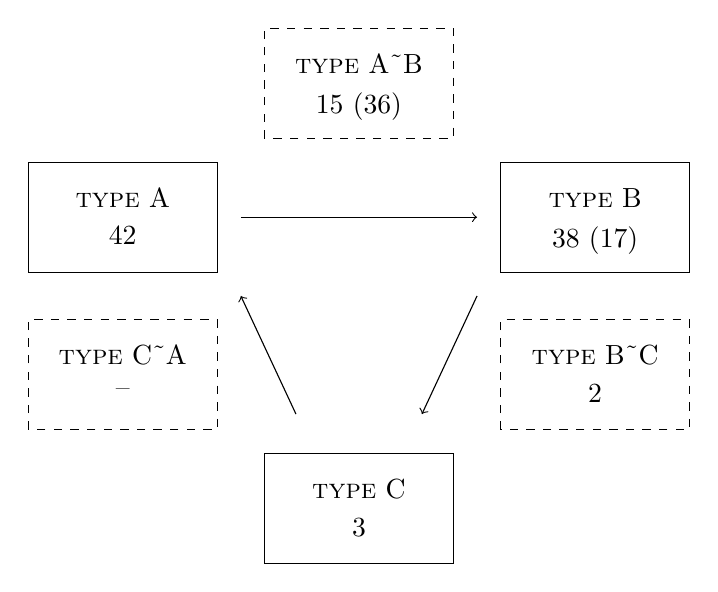
\begin{tikzpicture}
%\draw[help lines, dotted] (0,0) grid (12,8);
\draw [dashed] (4.8,6) rectangle (7.2,7.4); \node [above] at (6,6.7)
{\textsc{type} A\textasciitilde{}B}; \node [below] at (6,6.7) {15 (36)};
\draw (7.8,4.3) rectangle (10.2,5.7); \node [above] at (9,5) {\textsc{type}
B}; \node [below] at (9,5) {38 (17)}; \draw [dashed] (7.8,2.3) rectangle
(10.2,3.7); \node [above] at (9,3) {\textsc{type} B\textasciitilde{}C};
\node [below] at (9,3) {2}; \draw (4.8,.6) rectangle (7.2,2); \node [above]
at (6,1.3) {\textsc{type} C}; \node [below] at (6,1.3) {3}; \draw [dashed]
(1.8,2.3) rectangle (4.2,3.7); \node [above] at (3,3) {\textsc{type}
C\textasciitilde{}A}; \node [below] at (3,3) {\rule{0pt}{1ex}--}; \draw
(1.8,4.3) rectangle (4.2,5.7); \node [above] at (3,5) {\textsc{type} A};
\node [below] at (3,5) {42}; \draw [->] (4.5,5) -- (7.5,5); \draw [->]
(7.5,4) -- (6.8,2.5); \draw [->] (5.2,2.5) -- (4.5,4);
\end{tikzpicture}\caption{Stages of the NEC across the Bantu
sample}\label{fig:01-bantu-nec}\end{figure}\end{center} 
As can be seen in
\figref{fig:01-bantu-nec}, the majority
of existential negators across Bantu pertain to the `earlier' stages of the
cycle, thus adhering to cross-linguistically induced generalizations
regarding rate of frequency \parencites{Croft1991}{Veselinova2016}. This
tendency is arguably even stronger if it is taken into account that the
three C types and one of the B{\textasciitilde}C types of this figure are
plausibly the result of contact induced change involving one and the same
source language, i.e., \ili{Swahili}. A word of caution is warranted here
however, regarding the presentation of the data more generally but
specifically regarding the relationship between negative existentials of
the stable Type B and those of Type A{\textasciitilde}B. In many cases, our
sources have only provided examples with negative existential constructions
in the present tense. This has made it difficult to determine with
certainty whether a language really makes use of a negative existential of
Type B or A{\textasciitilde}B.\footnote{Of course, such a problem could
also hold for other contextual restrictions which are not revealed in the
data.} We therefore decided to use two numbers. The first number (without
parentheses) represents the liberal count which takes the absence of a
description of other means of negative existential predication as an
indication of a special Type B status of the negative existential marker in
question. The second number (in parentheses) represents the alternative,
more conservative count where the absence of examples of usage outside of
the present temporal domain is taken to indicate that the negative
existential is of Type A{\textasciitilde}B.

The following two sections each discuss one half of the cycle. In
\sectref{sec:1:5}, we focus on Type A and B and the transition processes
between these types. In \sectref{sec:1:6}, we address the rarer, additional
types and hence further developed stages within the cycle found in Bantu,
including those induced by contact with \ili{Swahili}. In \sectref{sec:1:6}, we also raise the question of meaning extensions of negative existentials in Bantu which are not necessarily connected to the NEC.

\section{From non-dedicated to dedicated negative existentials in Bantu}\label{sec:1:5}
In this section, we discuss instantiations of the first half of the NEC,
that is, A, B and A{\textasciitilde}B. As seen in \figref{fig:01-bantu-nec}
above, these three types/stages constitute the vast majority of
instantiations of the NEC in Bantu, in accordance with the observed general
cross-linguistic tendency \citep{Veselinova2016,Croft1991}.
\sectref{sec:1:5.1} discusses constructions which apply standard negation
to affirmative existential constructions, i.e. negative existentials of
Type A. \sectref{sec:1:5.2} continues with an account of dedicated negative
existentials, either as part of a Type A{\textasciitilde}B or a Type B
situation, and their evolution.

\subsection{Negative existentials using standard negation}\label{sec:1:5.1}
As can be seen in \figref{fig:01-bantu-nec}, a majority of negative 
existentials across Bantu are formed in a compositional fashion by applying 
standard negation strategies to the affirmative existential construction. That is, Type A negative existentials in \citegen{Croft1991} typology. Interestingly, although a majority of Bantu languages stick to the compositional formation of negative existentials, there is still a lot of variation in the expression of Type A negative existentials. This reflects the formal variation within the expression of both standard negation (\sectref{sec:1:2}), and affirmative existence (\sectref{sec:1:3}) in Bantu.

All instantiations of the negative existential of Type A across Bantu involve standard negation strategies. However, languages vary (both internally and externally) as to whether standard negation is applied to a non-dedicated or, as in the great majority (roughly three quarters) of the cases, dedicated affirmative existential. In the latter case, languages vary in terms of which specific type of dedicated affirmative existential is involved, thus prompting more fine-grained distinctions within the single category of Type A negative existentials.

An example of a Bantu language where standard negation is applied to a
non-dedicated existential construction is \ili{Swahili}. In
\REF{ex:swahili-pig}, the standard pre-initial negative marker is attached
to a type of existential predication which is described as under-specified
in relation to plain locational predication in \sectref{sec:1:3.1} (cf. the
Swahili examples in \REF{ex:swahili-agriculture-table}).
\ea\label{ex:swahili-pig} \langinfo{Swahili}{}{G42, Kanijo p.c. 2018}\\
\gll ha-yu-po nguluwe mw-enye ma-bawa\\ \textsc{neg-sm1-loc.cop16} 9.pig
1-having 6-wings\\ \glt `There is no pig with wings.' \z There are also
languages in which standard negation applies to the dedicated existential
constructions discussed in \sectref{sec:1:3.2}. Thus, Ikizu\il{Ikizu} and
Kisi\il{Kisi} are examples of standard negation combined with dedicated
locative-existential constructions. In the Ikizu case, the affirmative
existential involves an obligatory locative enclitic
\REF{ex:ikizu-relatives}, whereas the existential in Kisi is characterized
by a locative subject marker, as in \REF{ex:kisi-sardines}. Note that the
strategy used in standard negation in Kisi is a post-verbal negative
particle.  \ea\label{ex:ikizu-relatives} \langinfo{Ikizu}{}{JE402, Luke
1:61, \citealt[54]{Gray2013}}\\ \gll Ndora mʉ-bahiiri banyu ta-ree-ho wi
riina riyo!\\ look 18-2.blood.relative 2.\textsc{poss2pl}
\textsc{neg}-be-\textsc{loc}16 1.of 5.name 5.\textsc{dem}2\\ \glt`Look,
among your blood relatives there is no-one of that name!' \z
\ea\label{ex:kisi-sardines} \langinfo{Kisi}{}{G67,
\citealt[157]{Ngonyani2011}}\\ \gll n-dofi a-bhʊlile ku-yele he bhu-sipa
ma-gono agho\\ 1-fisherman \textsc{sm1}-say.\textsc{pfv} 17-be.\textsc{pfv}
\textsc{neg} 14-sardine 6-day 6.\textsc{dem}2\\ \glt `The fisherman said
there were no sardines in those days.' \z 
%
Similarly, standard negation may apply to affirmative existential
constructions of the comitative type.  Swahili\il{Swahili} is a case in
point. In addition to the non-dedicated existential construction
illustrated in \REF{ex:swahili-pig}, Swahili makes use of a dedicated
co\-mi\-ta\-ti\-ve-exis\-ten\-tial. The corresponding negative 
construction simply adds the standard pre-initial negative marker \textit{ha-}. Recall, that these constructions typically also involve locative marking, in this case the class 16 locative subject marker \textit{pa-}.  %
\ea\label{ex:swahili-mistake} \langinfo{Swahili}{}{G42,
\citealt[25]{KingeiNdalu2009}}\\ \gll ha-pa-na m-tu a-si-ye-fanya ma-kosa\\
\textsc{neg}-\textsc{sm}16-\textsc{com} 1-person
1-\textsc{neg}-\textsc{rel}1-make 6-mistake\\ \glt `There is no person who
does not make mistakes.' \z 
%
Some languages that are categorized as
belonging to Stage A because they employ standard negation strategies in
negative existential constructions, display minor irregularities. Since the
irregularities are typically attested in present tense contexts they could
be suggestive of the emergence of a dedicated negative existential.
Makwe\il{Makwe} is a case in point. One of the negative existential
strategies found in Makwe involves standard negation in combination with a
locative\slash existential predicate (\textit{-pali}) derived from the
univerbation of a class 16 object prefix \textit{-pa-} and the copula
\textit{-li} `be', as seen in \REF{ex:makwe-problem}.  The corresponding
affirmative construction also makes use of a locative\slash existential
predicate (\textit{-pwawa}) which, however, is most probably the result of
the merger of a class 16 object prefix \textit{-pa-} with the verb
\textit{-wa} `be' (rather than \textit{-li}), as seen in
\REF{ex:makwe-song}.  The locative\slash existential predicate
\textit{-pali} cannot be used in affirmative contexts. It only occurs in
negative present tense contexts. Other temporal contexts make use of
\textit{-pwawa} in combination with standard negation \REF{ex:makwe-sugar}.
%
\ea\label{ex:makwe-problem-song-sugar} \langinfo{Makwe}{}{P231,
\textit{fieldnotes}, \citealt[375]{Devos2008}} 
\ea\label{ex:makwe-problem}
\gll a-ya-pa{\'a}li ma-tati{\'\i}zo\\ \textsc{neg-sm}6-exist 6-problem\\
\glt `There are no problems.' 
\ex\label{ex:makwe-song} \gll u-ni-pw{\'a}awa
mw-{\'\i}imbo\\ \textsc{sm3-pfv}{}-exist  3-song\\ \glt `There is a song.'
\ex\label{ex:makwe-sugar} \gll a-ku-na-pwaw-{\'\i}ije na suk{\'a}ali\\
\textsc{neg-sm17-pst}-exist-\textsc{pfv} with 9.sugar\\ \glt `There was no
sugar available.' \z\z 
%
Another example comes from \ili{Shangaji}. Shangaji
has a dedicated locative-ex\-is\-ten\-tial strategy marked by an obligatory
locative enclitic, as seen in \REF{ex:shangaji-mosquito}. 
This can be negated through standard negation which
involves the pre-initial negative marker \textit{kha-}, as in
\REF{ex:shangaji-star}. However, the copula verb \textit{-wa}, present in the
affirmative construction, is reduced to zero in the negative construction,
thus turning the locative enclitic into a locative copula.\footnote{Note
that the affirmative existential construction makes use of a series of
locative demonstrative enclitics (\textit{-pho}, \textit{-kho} and
\textit{-mo}) whereas the negative existential construction uses a series
of locative relative enclitics (\textit{-vo}, \textit{-wo} and
\textit{-mo}).} \ea\label{ex:shangaji-mosquito-star}
\langinfo{Shangaji}{}{P312, Devos, \textit{fieldnotes}}
\ea\label{ex:shangaji-mosquito} \gll le{\'e}lo zi-wa{\'a}-pho
pwil{\'\i}mw{\'\i}ithi\\ today \textsc{sp}10-be-\textsc{loc}16
10.mosquito\\ \glt `Today there are (a lot of) mosquitos.'
\ex\label{ex:shangaji-star} \gll le{\'e}lo kha-z{\'\i}-w{\'o}
tthondd{\'o}owa o-t{\'u}ulu\\ today \textsc{neg-sp10-loc17} 10.star
17-above\\ \glt `Today there are no stars in the sky.' \z\z

\subsection{The rise of dedicated negative existential
strategies}\label{sec:1:5.2} 53 of the languages -- more than half of our
sample -- can be considered to belong to Type B or Type A{\textasciitilde}B
of the NEC, thus having a dedicated negative existential strategy which
does not merely involve the application of standard negation to an
affirmative existential construction. In this section, we first explore the
etymology of dedicated negative existential markers across the Bantu
family. We then go on to address the transition between stage A and B,
i.e., the emergence of dedicated negative existentials in Bantu. 

\subsubsection{Dedicated negative existential
constructions}\label{sec:1:5.2.1} Dedicated negative existential
constructions in Bantu are often marked by inherently negative lexemes in
combination with locative marking. There are two main lexical sources
involved in such dedicated negative existential constructions: verbs and
adjectives\slash adverbs. Both categories can be etymologically linked to a
negative source meaning, which adheres to a common cross-linguistic pattern
\citep{Veselinova2013}. Two geographically more restricted patterns have
also been identified. The first concerns non-verbal predication whereby
the noun referring to the figure is followed by a negative particle
dedicated to the expression of negative existence (and other non-verbal
predication types). The second involves locative subject marking in
combination with a verbal enclitic with an as yet unclear etymology. This
section takes a closer look at all four more or less recurrent sources, starting with the least
unexpected one.

Bantu languages commonly recruit inherently negative verbs as negators (see \citealt{Givon1973}; \citeyear[382--383]{Givon2001}). This is typically the case in prohibitive propositions and, by extension, other types of more marked verbal negation (see e.g. \citealt{Bernander2018}, \citealt{DevosOlmen2013}, 
\citealt{Guldemann1999}, \citealt[191--193]{Nurse2008}, and also the brief discussion in \sectref{sec:1:2} of this paper). Our investigation shows that lexical verbs of similar denotations are often also recruited as negative existential markers in Bantu, always in combination with locative marking. This can be seen in the examples below from \ili{Ruwund} and \ili{Kagulu}.
\ea\label{ex:ruwund-nothing}
\langinfo{Ruwund}{}{L53, \citealt[839]{Nash1992}}\\
\gll p-{\`\i}{\`\i}kil c{\^o}m\\
	\textsc{sm}16-not.be 7.thing \\
\glt `There is nothing there.'
\z
\ea\label{ex:kagulu-people}
\langinfo{Kagulu}{}{G12, \citealt[167]{Petzell2008}}\\
\gll kw-ichak-a wa-nhu\\
	\textsc{sm}17-be.without-\textsc{fv} 2-people\\
\glt `There are no people.'
\z
Arguably, similar processes of semantic bleaching apply to those verbs
recruited as negative existentials as to those becoming negative
auxiliaries in marked negation types. An important difference is the
construction as a whole, since negative verbs which become negative existentials are always inflected with locative subject markers. Thus, locative marking is a persistent feature in both affirmative and negative existential constructions across Bantu. This adheres to the close contiguity in meaning between location and existence given the basic conceptualization that an entity occupying a space also exists (\citealt[407]{Lakoff1987}; see also \citealt{Gaeta2013}, \citealt{Koch2012}) and by analogy does not exist if it is not occupying a space.

The most typical original meaning of a negative existential verb is `be
without, lack', as in the example from \ili{Kagulu} in
\REF{ex:kagulu-people} above. Other examples include \textit{-vʊla} and
\textit{-bhʊl{\'a}} in \ili{Kinga} (G65) and \ili{Bende} (F12) respectively
(from Proto-Bantu *\textit{-bʊd}- `lack; be lacking; be lost'
\citep{BastinCoupez2002}), \textit{-gaya} `lack' in \ili{Bena} (G63) and
\ili{Hehe} (G62), and \textit{-hela} `lack' in \ili{Pogolo} (G51) and
\ili{Ndamba} (G52). It is worth noting that the meanings `be without, lack'
express the polar denotation of the affirmative comitative-existential
strategy, discussed in \sectref{sec:1:3}. This suggests that this
conceptualization of existentials, typical for Bantu languages, applies to
the formation of negative existentials even beyond those of Type
A.\footnote{Interesting in this regard is \ili{Gogo} (G11) which appears to
form negative existentials by applying standard negation to a
comitative-existential construction, whereas it employs affirmative
constructions of the locative-existential type.} 
% 
Arguably, it also supports the suggestion of \citet{Veselinova2013} that
negative existentials represent a separate functional domain from
affirmative existentials, making statements about the absense of something
rather than negating an existence, and thus does not have to be secondary
formations to affirmative existentials. 
%
More generally, this fact can be seen to reflect the conceptual interaction
and semantic contiguity not only between location and existence, but also
between possession and existence both synchronically and diachronically
\parencites(see e.g.)(){Koch1999}{Koch2012}{Heine1997}[see
also][]{Veselinova2013}.

This being said, however, there are also lexical sources which do not
denote negative possession, but which still arguably have an inherently
negative meaning. In several cases the source is a lexical verb simply
meaning `not be', in accordance with a more general cross-linguistic
tendency %
%
\parencites(see)(){Veselinova2013b-Bantu}{Veselinova2016}. One such example
is the
negative existential \textit{t{\`\i}ti} in \ili{Duala} (A24), which
according to \citet{Ittmann1939,Ittmann1976} stems from an archaic verb
\textit{t{\`\i}t{\'a}} `not be, not exist' inflected for the perfect.
Another example is \textit{-{\`\i}{\`\i}kil} in \ili{Ruwund}, as seen in
\REF{ex:ruwund-nothing} above. \ili{Lusoga} (JE16), \ili{Bena} (G63) and
\ili{Vwanji} (G66) appear to make use of a reflex of the
reconstructed verb *\textit{-g{\`\i}d-} `abstain from, avoid, refuse'. A
final example of a negative existential derived from a negative verbal
source in Bantu is \textit{-fwa} `die' which is used in both \ili{Kisanga}
(L35) and \ili{Kaonde}, as illustrated in \REF{ex:kaonde-corn}.
\ea\label{ex:kaonde-corn} \langinfo{Kaonde}{}{L41,
\citealt[30]{Foster1960}}\\ \gll k{\'e}sha tu-k{\'e}kala na ma-t{\'a}ba
l{\'e}lo ka-fw{\'a}-ko\\ tomorrow \textsc{sm1pl}-be \textsc{com}
\textsc{ncp}6-corn today \textsc{neg}-die-\textsc{loc}17\\ \glt `Tomorrow
we shall have corn, today there is none.' \z 
%
In total, 22 languages --
almost a quarter of our sample -- resort to inherently negative verbs in
the formation of negative existential constructions, whether this is as the
sole marker or together with other strategies.

Another frequent and widespread source of negative existentials in our
sample of Bantu languages is not a verb but rather an adjectival or
adverbial form meaning `empty' (and\slash or with similar meanings). Of the
15 attestants, the most typical case involves reflexes of the Proto-Bantu
stem *\textit{-t{\'ʊ}p{\'ʊ}} `only, empty, vain'
\parencite{BastinCoupez2002,Angenot1977} in combination with a locative
class marker. Examples \REF{ex:kwangali-water} and \REF{ex:ndengeleko-fish}
from \ili{Kwangali} and \ili{Ndengeleko} exemplify this pattern. Note that
there is a mismatch in class agreement between the \textit{-t{\'ʊ}p{\'ʊ}}
form and the locative nominal argument in \REF{ex:ndengeleko-fish}. This
lack of automatic agreement suggests that the referential locative reading
has been lost, which points to a further decategorialization of the
construction as a whole.  \ea\label{ex:kwangali-water}
\langinfo{Kwangali}{}{K33, \citealt[108]{Dammann1957}}\\ 
\gll mo-ru-pasa m{\op}u{\cp}-tupu mema\\ 
18-11-bowl 18-empty 6.water\\ \glt `In the bowl there is
no water.' \z \ea\label{ex:ndengeleko-fish} \langinfo{Ndengeleko}{}{P11,
\citealt[284]{Strom2013}}\\ \gll n-t{\'ʊ}p{\'ʊ} oomba ku-lw-{\'\i}i\\
18-empty 9/10.fish 17-11-river\\ \glt `There is no fish in the river.' \z
Nine languages of our sample have a negative existential involving
*\textit{-t{\'ʊ}p{\'ʊ}} with a locative prefix. The other 7 
%\todo{maybe rather `seven' than `7'?} 
languages not discussed above are summarized in
\REF{ex:neg-derived-empty}.  
%
\begin{exe}\ex\textbf{Languages with a
negative existential derived from *\textit{-tʊpʊ}}\\
\begin{tabularx}{\textwidth}{@{}lll@{}} 
F.12 	&Bende &\textit{h{\'a}tuh{\'u} {\textasciitilde} k{\'u}tuh{\'u}}\\ 
F.22 &Nyamwezi &\textit{hadʊhʊ {\textasciitilde} ndʊhʊ} \\ 
G.35 	&Luguru
&\textit{muduhu}\\ L.33 	&Luba 		&\textit{patupu {\textasciitilde}
kutupu {\textasciitilde} mutupu} \\ L.35 	&Kisanga 		&\textit{patupu
{\textasciitilde} kutupu {\textasciitilde} mutu(pu)}\\ P.13 	&Matumbi
&\textit{patʊpʊ {\textasciitilde} kutʊpʊ {\textasciitilde} ntʊpʊ}\\ P.14
&Ngindo 		&\textit{haduhu}\\
\end{tabularx}\label{ex:neg-derived-empty} \end{exe} 
%
Some other words with
roughly the same meaning have also been recruited into negative existential
constructions. This can be seen in the form \textit{-bule} which is found
in \ili{Swahili} (G42) and which is thought to derive from the \ili{Arabic}
word \textit{bure} [\textarab{برع{}}] `bestow of free will', and, by extension
`vain' (\citealt[42]{Johnson1939}; \citealt[48]{TUKI2014}). A similar form,
presumably borrowed into the language from \ili{Swahili}, can also be seen in
\ili{Kami}, a highly endangered language spoken in Tanzania which has been
in sustained contact with Swahili.  \ea\label{ex:kami-sweden}
\langinfo{Kami}{}{G36, \citealt{PetzellAunio2016}}\\ \gll Sweden ha-bule
tangawizi\\ Sweden 16-\textsc{neg.ex} 9/10.ginger\\ \glt `There is no
ginger in Sweden.' \z Another example is the form \textit{-waka} `only,
vain, naked' recruited as a negative existential marker in \ili{Ngoni}
(N.12) and also in \ili{Manda}, as exemplified in \REF{ex:manda-money}.
\ea\label{ex:manda-money} \langinfo{Manda}{}{N11,
\citealt[335]{Bernander2017}}\\ \gll s{\'e}nde pa-w{\'a}ka? \\ 9/10.money
16-empty\\ \glt `Is there no money (left)?' \z 
%
In 10 languages, spoken in parts of Gabon, Congo and the Democratic
Republic of Congo (DRC), negative existence is expressed by non-verbal
predication, i.e., the figure is simply followed by a negative particle.
\ili{Duma} is a case in point.  The copula \textit{li} which is present in
the affirmative existential construction in \REF{ex:duma-pig} is not
attested in the negative existential construction in \REF{ex:duma-porter}
and, whereas standard negation involves both pre-initial \textit{ka-} and
clause-final \textit{vɛ} \REF{ex:duma-kill}, only the latter is used for
the expression of negative existence.  
%
\ea\label{ex:duma-pig-porter-kill} \langinfo{Duma}{}{B51}
\ea\label{ex:duma-pig} affirmative existential \citep[148]{Adam1954}\\ 
\gll mungubili mu li i {tswa ngundu}\\ 
1.pig \textsc{sm1} \textsc{cop} \textsc{loc} garden\\ 
\glt	`There is a pig in the garden.'
\ex\label{ex:duma-porter} negative existential \citep[148]{Adam1954}\\ \gll
ba{\~a}ti bo vɛ\\ 2.porter \textsc{pers}.2 \textsc{neg}\\ \glt 	`There are
no porters.' \ex\label{ex:duma-kill} standard negation
\citep[144]{Mickala1988}\\ \gll bes{\'u} ka-li-b{\'o}ma m{\'u}tu vɛ\\
\textsc{pers.1pl} \textsc{neg-sm1pl}-kill 1.person \textsc{neg}\\ \glt 	`We
do not kill the man.' \z\z 
%
Languages in this area typically have a
discontinuous or double standard negation strategy which combines a
pre-verbal, pre-initial or post-initial negative marker with a second
post-verbal (either immediately following the verb or in clause-final
position) negative marker \citep{DevosAuwera2013}. In some languages, the
negative marker used for the expression of negative existence is identical
to the standard post-verbal negative marker, as seen in the \ili{Duma}
example \REF{ex:duma-pig-porter-kill} and also in
\REF{ex:nduumo-honey-porter} from \ili{Nduumo} (cf. also
\sectref{sec:1:5.2.2}).  \ea\label{ex:nduumo-honey-porter}
\langinfo{Nduumo}{}{B63, \citealt[141, 148]{Adam1954}} \ea standard
negation\\ \gll bisi ka li dji buyu ng'i\\ \textsc{pers.1pl} \textsc{neg}
\textsc{sm1}pl eat honey \textsc{neg}\\ \glt `We have not eaten the honey.'
\ex negative existential\\ \gll abiti ng'i\\ porter \textsc{neg}\\ \glt
`There are no porters.' \z\z However, in a few languages the existential
negator formally differs from the post-verbal standard negator, as shown by
the examples in \REF{ex:mbete-honey-porter} from the closely related
language \ili{Mbete}.

\ea\label{ex:mbete-honey-porter} \langinfo{Mbete}{}{B61, \citealt[141,
148]{Adam1954}} \ea standard negation\\ \gll bisi le ha dja bvugi ng'i\\
\textsc{pers.1pl} \textsc{sm1pl} \textsc{neg} eat honey \textsc{neg}\\ \glt
`We have not eaten the honey.' \ex negative existential\\ \gll abiti kali\\
porter \textsc{neg}\\ \glt 	`There are no porters.' \z\z It should be noted
that the \ili{Nduumo} standard post-verbal negative marker in
\REF{ex:nduumo-honey-porter} can be replaced by the negative marker
\textit{onyang'a}, i.e., \textit{abiti onyang'a} `there are no porters'.
The semantics and the usage range of \ili{Mbete} form \textit{kali} and the
Nduumo form \textit{onyang'a} are not entirely clear. \citet[114,
171]{BitonAdam1969} give the translation equivalents `no' and `none, nil',
respectively, suggesting an origin in a negative answer particle in Mbete
and a negative indefinite pronoun in Nduumo. However, meanings reminiscent
of *\textit{-t{\'ʊ}p{\'ʊ}} are attested as well. As can be seen in
\REF{ex:mbete-nduumo-empty}, both elements can be used to express `empty'.
\ea\label{ex:mbete-nduumo-empty} 
\ea\langinfo{Mbete}{}{B61, \citealt[649]{BitonAdam1969}}\\ 
\textit{djyala kali}\\ 
\glt `empty handed'
\ex\langinfo{Nduumo}{}{B63, \citealt[649]{BitonAdam1969}}\\ 
\textit{bvyala onyang'a}\\ 
\glt `empty handed' \z\z 
%
Whether the existential negator is identical or
not to the post-verbal standard negator, we consider this particular type
of negative existential construction as specialized, i.e., of type
A{\textasciitilde}B (if only used in the present tense) or of type B (and
plausibly even type B{\textasciitilde}C or C if the existential negator
indeed spreads to standard negation). In \sectref{sec:1:6.3} we discuss the
possible enrolment of these existential negators in the expression of
standard negation through a Jespersen Cycle. \sectref{sec:1:6.1} addresses
the possible usage extension of these existential negators to other types
of non-verbal predication and vice versa.

Finally, there is a small set of only 4 languages spoken in a contiguous
area in Malawi and Zambia where negative existence is expressed by adding
an enclitic to affirmative existential predication of the locative
existential type. The enclitics are \textit{-je} in \ili{Tumbuka} (N21),
\textit{-be} in \ili{Chewa\slash Nyanja}\il{Nyanja} (N31),
\textit{-ye}/\textit{-ve} in \ili{Nsenga} (N41) and \textit{-je} in
\ili{Nyungwe} (N43). The etymology of these arguably cognate forms is as
yet unclear to us. In at least the Chewa\slash Nyanja case, the enclitic
displays a curious polysemy between expressing negative existence\slash
possession when combined with the copula \textit{-li}/\textit{-ri}, and the
phasal meaning `still' when combined with a verb or even a noun 
%
\parencites[116]{Hetherwick1916}[97, 99]{Watkins1937}[209]{Price1953}
[116, 205, 279]{StevickHollander1965}[20--21]{Paas2004}
[60, 68]{Mchombo2004}[150, 153, 161]{Kiso2012}.  
%
\ea\label{ex:chewa-nyanja-orange-sleep} \langinfo{Chewa\slash Nyanja}{}{N31,
\citealt[117, 205, 279]{StevickHollander1965}}\il{Nyanja} \ea negative possession\\
\gll ndi-li-be ma-lalanje\\ \textsc{sm1sg}-be-\textsc{neg/poss} 6-orange\\
\glt 	`I don't have any oranges.' \ex negative existential\\ \gll kuno
ku-li-be ma-lalanje ambili\\ 17.\textsc{dem1} 17-\textsc{cop-neg/exist}
6-oranges 6.many\\ \glt `There aren't many oranges around here.' \ex
persistive\\ \gll a-ku-gon-a-be\\ \textsc{sm1-prs}-sleep-\textsc{per}\\
\glt `He's still sleeping.' \z\z 
%
\citet[279]{StevickHollander1965} express
some doubts about the tonal identity between negative existential
\textit{-be} and persistive \textit{-be}. This, together with the fact that
`still' does not appear to be a common source of negative existence or vice
versa (\citealt{HeineGuldemann1993} and \citealt{HeineKuteva2002}, for
example, do not mention a conceptual shift in either direction), might
suggest that homonymy rather than polysemy is at play here. However, the
semantic connection between `still' and `empty' which, as has been shown
above, is a common source of negative existentials in Bantu, is confirmed
by data from \ili{Tumbuka} (N21). Tumbuka has an element \textit{waka},
cognate with \ili{Manda} and \ili{Ngoni} \textit{-waka}, which is used
adverbially to express `empty(ly), vain' and in combination with the copula
\textit{-ri} to express `still', as illustrated in
\REF{ex:tumbuka-empty-persist}.  \begin{exe}
\ex\label{ex:tumbuka-empty-persist} \langinfo{Tumbuka}{}{N21,
\citealt[120--121]{Young1932}} \begin{xlist} \ex `empty, vain'
\begin{xlist} \ex{\gll w-iz-a waka\\ \textsc{sm}1-come-\textsc{pfv} empty\\
\glt `S/he has come empty-handed / for no particular purpose.'} \ex{\gll
w-a-gon-a waka\\ \textsc{sm}1-\textsc{pst}-sleep-\textsc{fi} empty\\ \glt
`S/he slept without food / without the evening meal.'} \end{xlist}
\ex{persistive\\ \gll zuwa li-ri waka\\ 5.sun \textsc{sm}5-\textsc{cop}
still\\ \glt `The sun is still shining / There is still daylight.'}
\end{xlist} \end{exe} 
%
This might suggest that the lexical source of \textit{-be} is similarly an
element expressing `empty' and that this element has developed multiple
grammatical functions.

As a final note, it should be mentioned that we are even less sure about
the etymology of other instances of Bantu negative existentials in our
sample. This might, of course, have had an effect on the outcome presented in this section.

\subsubsection{Variation between standardly negated and dedicated negative
existentials}\label{sec:1:5.2.2} In accordance with cross-linguistic
tendencies \citep{Veselinova2016}, there are several examples of Bantu
languages in the transition stage A{\textasciitilde}B where a negative
existential may be expressed both through applying standard negation
strategies (to either a non-dedicated or a dedicated affirmative
existential) or, alternatively, a dedicated negative existential marker. As
is typical in these cases, the usage of the specialized existential is
confined to the present, standard negation being employed in other temporal
contexts \parencites{Veselinova2013}{Veselinova2016}. \ili{Luba} is a case in
point. In the present tense, Luba can make use of a dedicated negative
existential strategy involving \textit{-tupu}, a reflex of
*\textit{-t{\'ʊ}p{\'ʊ}}, discussed in the previous section. In all other
temporal contexts, standard negation is applied to the affirmative
existential of the locative-existential type, as can be seen in
\REF{ex:luba-knife-salt}.  \ea\label{ex:luba-knife-salt}
\langinfo{Luba}{}{L33, \citealt[126]{Beckett1951}} \ea\gll le ku-di
lu-pete? ku-tupu-lo\\ \textsc{int} 17-\textsc{cop} 11-knife? 17-empty-11\\
\glt 	`Is there a knife? There is not.' \ex\gll ke-kwa-di-po mwepo nansha
mu-tyetye\\ \textsc{neg-17.pst-cop-neg} 3.salt even 3-little\\ \glt
`There was not even a little salt.' \z\z \ili{Ombo} constitutes a similar
case. In the present tense, the dedicated inherently negative verb
\textit{-{\'a}fa} `not be' is recruited for the expression of negative
existence \REF{ex:ombo-knife}, whereas other temporal contexts resort to
standard negation applied to an affirmative existential of the
comitative-existential type, as seen in \REF{ex:ombo-lion}.
\ea\label{ex:ombo-knife-lion} \langinfo{Ombo}{}{C76,
\citealt[30]{Meeussen1952}} \ea\label{ex:ombo-knife} \gll k-{\'a}fa
lʊ-kula\\ \textsc{sm}17-not.be 11-knife\\ \glt 	`There is no knife.'
\ex\label{ex:ombo-lion} \gll ku-t{\'a}-{\'\i}k{\'a} la-ns{\'\i}mba\\
\textsc{sm}17-\textsc{neg}-be.\textsc{pst} \textsc{com}-10.lion\\ \glt
`There were no lions.' \z\z 
%
For 18
of our languages (almost a fifth), the sources claim that such a situation
holds. However, given the fact that not many sources provide an extensive
account of the expression of negative existence, let alone the variation
within, it is likely that this number is actually higher. Furthermore,
dedicated negative existentials might have emerged after the publication of
the sources, seeing that negative existentials typically are subject to
renewal \citep{Veselinova2016} and the verbal systems of Bantu languages in particular are
characterized by rapid innovation and change \citep[25]{Nurse2008}. An
indication of such a situation, with what appears to be an emerging
dedicated negative existential, comes from \ili{Kinga}, a language which
can be described as belonging to variationist Type\slash Stage
A{\textasciitilde}B. In Kinga, a negative existential proposition may be
produced by employing standard negation strategies, as in
\REF{ex:kinga-soda-1}. Alternatively, a dedicated negative existential
marker may be used, derived from the inherently negative verb
\textit{-vʉla} `lack' and inflected with a locative subject marker, as in
\REF{ex:kinga-soda-2}.  
%
\ea\label{ex:kinga-soda} \langinfo{Kinga}{}{G67,
Eaton p.c. 2017} \ea\label{ex:kinga-soda-1} 
\gll ni-pa-li i-soda \op{\textasciitilde}/nɩpali ɩsoda\cp\\ 
\textsc{neg-sm16-cop} \textsc{9-}soda\\
\glt 	`There's no soda.' \ex\label{ex:kinga-soda-2} \gll kʊ{}-vʊl-a
soda\\ \textsc{sm}17-lack-\textsc{fv} 9.soda\\ \glt 	`There is no soda.'
\z\z 
%
However, there is no account at all of the negative existential use of
\textit{-vʉla} in the grammar on \ili{Kinga} by \citet{Wolff1905}. What is
more, according to Helen Eaton (p.c.), \textit{-vʉla}
with a negative existential only turns up five times in the New Testament,
whereas the version with standard negation is far more frequent. Similarly,
the neighboring and closely related language \ili{Bena} is claimed to
employ standard negation with the affirmative existential construction
\citep[378]{Morrison2011}. However, going through an annotated collection
of Bena narratives \citep{Eaton2015a}, we found not only one, but two
negative existential markers transparently derived from inherently negative
verbs plus locative marking.
%\footnote{It actually appears that the negative
%existentials in these examples consist of the stacking of two locative
%markers. This is not unheard of for other construals of dedicated
%(negative) existentials in Bantu, however.} 
%
In fact, there is a set of
languages spread across the Bantu speaking area which appears to make use
of several dedicated negative existentials. Other examples of languages
with several dedicated negative existentials are the Mozambican variety of
\ili{Ngoni}, \ili{Bende} in Tanzania, \ili{Luba} in DRC and \ili{Lusoga} in
Uganda (cf. \tabref{tab:1:1} in the Appendix). Unfortunately, there is
seldom any elaboration on the functional differences between these various
markers. In the case of \ili{Bena}, however, there might be dialectal or
other lectal differences at play, \ili{Bena} being characterized by
relatively extensive language-internal variation (cf.
\citealt[30--35]{Morrison2011}; \citealt{Morrison2015};
\citealt{Mitterhofer2013}).

\section{Further processes of change}\label{sec:1:6}
%
The focus of this section is the later language types and stages of the NEC
as reflected in the Bantu sample. Specifically, we look at types\slash stages
where the negative existential marker has expanded into the domain of
standard (verbal) negation. As can be deduced from
\figref{fig:01-bantu-nec} in \sectref{sec:1:4}, this does not seem to be 
very common in the Bantu languages. There is a possibility that some
of the illocutionary particles hypothesized by \citet{Guldemann1999} to
have developed into standard negation markers, as described in
\sectref{sec:1:2}, ultimately stem from negative existential markers.
However, we have failed to find any indications of such a scenario in our
data. In fact, it seems that in those cases where the negative existential
marker has acquired an extended function as a standard (verbal) negator in
Bantu, there are typically specific socio-linguistic factors such of
language contact at play. Such a case is addressed in
\sectref{sec:1:6.4}. First, however, we discuss usage extensions of the
negative existential marker outside of verbal negation
(\sectref{sec:1:6.1}). Then we turn to usage extensions involving marked
negation types (\sectref{sec:1:6.2}) and finally a possible case of
intertwinement between the negative existential cycle and the Jespersen
Cycle is discussed (\sectref{sec:1:6.3}).

\subsection{Extensions of negative existentials outside of verbal
negation}\label{sec:1:6.1}
%
A first usage extension concerns the cross-linguistically well-attested
development of negative answer particles (`no') and negative indefinites
(`no\-thing'\slash `no\-bo\-dy') out of negative existential forms
\parencites(see)()
{Schwegler1988}{Croft1991}{Veselinova2013}{Veselinova2014}{Veselinova2016}.
Instantiations of such a change from internal negator into external negator
are found at least in \ili{Ombo} (C76), \ili{Nyamwezi} (F22), \ili{Ngoni}
(N12), \ili{Matumbi} (P13) and \ili{Yao} (P21).

In \ili{Yao}, \textit{ngapagwa} `nothing, no one, never' is derived from a
negative existential form involving standard negation applied to an
existential predicator \textit{-pagwa} which is itself derived from a
merger between the locative object prefix \textit{-pa-} and the light verb
\textit{-gwa} `fall, occur' (\citealt[72]{Sanderson1922},
\citealt[174]{Whiteley1966}). Compare the examples in
\REF{ex:yao-want-game}.
%
\ea\label{ex:yao-want-game}\langinfo{Yao}{}{P21,
\citealt[72]{Sanderson1922}} 
\ea\gll m-ku-saka chichi? ngapagwa\\
\textsc{sm2pl-prs}-want what? nothing\\ \glt 	`What do you want?
Nothing.' \ex\gll nyama nga-ni-si-pagwa\\ 9.game
\textsc{neg-pst-sm}9-exist\\ \glt 	`There was no game.' \z\z 
%
Another
example of this usage extension can be seen in \ili{Matumbi} where the
negative answer particle \textit{kutupo} `no', exemplified in
\REF{ex:matumbi-kibata}, is clearly related to the negative existential
form, which can be seen in \REF{ex:matumbi-rain}.
\ea\label{ex:matumbi-kibata-rain} \langinfo{Matumbi}{}{P13,
\citealt[46]{Krumm1912}, \citealt[304]{Odden1996}}
\ea\label{ex:matumbi-kibata} \gll kutupo, ba-bi Kibata\\ no \textsc{sm}2-be
Kibata\\ \glt 	`No, they are in Kibata.' \ex\label{ex:matumbi-rain} \gll
ul{\'a}a ndʊp{\'ʊ}\\ 9.rain 18.vain\\ \glt 	`There is no rain.' \z\z
Similarly, in \ili{Ombo}, the negative existential form \textit{k{\'a}fa}
`there is not', consisting of a class 17 subject prefix \textit{ku-} and
the inherently negative verb \textit{-áfa} `not be', can be used as a negative
answer particle expressing `no' \citep[30]{Meeussen1952}.

Another type of usage extension relates to the fact that negative
existentials, negative plain locational clauses and negative possessives
are often marked in similar ways in Bantu languages. As touched upon
earlier in \sectref{sec:1:5.2.1}, there is a conceptual closeness, and
consequently a semantic contiguity, between such expressions which can be
observed more generally across languages. In Bantu, this conceptual
closeness is reflected in both affirmative and negative existential
constructions. Dedicated affirmative constructions are typically of the
locative or the comitative\slash possessive type. Moreover, locative marking is a
salient feature in both types of existential construction. This is also
true for dedicated negative existential constructions which furthermore
often involve lexical items with the meaning `lack, be without'.
\citet{Heine1997} and \citet[241--242]{HeineKuteva2002} postulate a
unidirectional pathway going from possessive predicates to existential
constructions. However, it is interesting to note that there are also
examples of the reverse pathway in our data, i.e., from negative
existential to negative possessive. That this is indeed the case can be
deduced from the transparent locative marking and lexical meanings involved
in the possessive constructions in question. Tanzanian \ili{Ngoni} can be
used to illustrate this. Just like its neighbour and closest relative
\ili{Manda} (discussed in \sectref{sec:1:5.2.1}, example
\REF{ex:manda-money}) Ngoni expresses negative existentials through a
construction consisting of a locative prefix attached to a lexeme
\textit{waka} originally meaning `empty, naked, only'. However, as can be
seen in \REF{ex:ngoni-knife}, in \ili{Ngoni} it is also possible to express
negative possessive propositions with the negative existential, merely by
the addition of a subject possessor.
%
\ea\label{ex:ngoni-knife} \langinfo{Ngoni}{}{N12,
\citealt[32]{Ebner1939}}\\ \gll ne' kwawaka chi-pula\\ \textsc{pers}.1sg
\textsc{neg.ex} 7-knife\\ \glt 	`I don't have a knife.' \z
%
\citet{Koch2012} discusses similar affirmative constructions in
\ili{Mandarin}, a to\-pic-pro\-mi\-nent language (as are the Bantu
languages). He suggests that the possessive reading stems from the
introduction of a second, thematic participant, introduced as a topic.
Thus, to paraphrase example \REF{ex:ngoni-knife} above, resulting in a
construction which roughly reads as `as for me, there is no knife'. The
introduced topic has then been reinterpreted (and conventionalized) as a
possessor, the existential pivot as the possessee and consequently the
whole existential construction as a construction expressing possession.
Although further and more thorough investigation is needed, this
explanation seems to hold for negative existentials becoming negative
possessives in Bantu languages.

This being said, when a language uses one and the same (dedicated) strategy
for the negation of possessive, plain locational and existential clauses
and the etymology of the particular strategy is unclear, it is hard to
decide from where the strategy started out. \ili{Tetela} presents such a
case. As can be seen in \REF{ex:tetela-chief-dwelling-work}, the invariable \textit{ke{\'e}ma} (different from standard
negation which involves a pre-initial or a post-initial negative marker) is
used for the negation of plain locational \REF{ex:tetela-chief}, possessive
\REF{ex:tetela-dwelling} and existential clauses \REF{ex:tetela-work}.
\ea\label{ex:tetela-chief-dwelling-work}\il{Tetela}
\langinfo{Tetela}{}{C71, \citealt[100, 102]{Labaere1970}}
\ea\label{ex:tetela-chief} \gll ow{\'a}nji ke{\'e}ma-k{\'ɔ}\\ 1.chief
\textsc{neg-loc}17\\ 
\glt 	`The chief is not there.'
%
\ex\label{ex:tetela-dwelling} 
\gll dim{\'\i} ke{\'e}ma lang{\'e}l{\'o} l{\'e}ngo\\ 
\textsc{pers.1sg} \textsc{neg} with\_village there\\ \glt 	`I
do not have a dwelling there.' \ex\label{ex:tetela-work} \gll ke{\'e}ma
olemp ɛl{\'ɔ}\\ \textsc{neg} work today\\ \glt 	`There is no work today.'
\z\z The etymology of \textit{ke{\'e}ma} is unclear. It is described as an
invariable, expressing `no, not, nothing, there is nothing (to say, to
ask)' \citep[155]{Hagendorens1957} but as explained above, such meanings
could also have derived from its use as a negative existential marker.
Languages like \ili{Nduumo}, \ili{Mbete} and \ili{Duma} similarly use one
and the same (dedicated) strategy for the negation of locational,
possessive and existential clauses. This is illustrated in
\REF{ex:mbete-bush-food-cassava} for \ili{Mbete}. Again, the etymology of
the dedicated negator \textit{kali} cannot be ascertained (cf. also the
discussion in \sectref{sec:1:5.2.1}).
%
\ea\label{ex:mbete-bush-food-cassava} \langinfo{Mbete}{}{B61, \citealt[141,
148]{Adam1954}} 
\ea\gll bisi ho {tca cwaha} kali\\ \textsc{pers.1pl}
\textsc{loc}16 bush \textsc{neg}\\ 
\glt `We are not in the bush.'
\ex\gll me bila kali\\ 
\textsc{pers.1sg} food \textsc{neg}\\ 
\glt 	`I do not have food.' 
\ex\gll ekwo kali\\ cassava \textsc{neg}\\ 
\glt `There is no cassava.' \z\z

\subsection{From negative existential to other marked negation types: the
Ruwund case}\label{sec:1:6.2}
%
In \ili{Ruwund}, negative existence can be expressed by applying standard
negation, consisting of the discontinuous negative marker
\textit{ka-\ldots{}-p}, to the affirmative existential construction. This
is illustrated in \REF{ex:ruwund-problem-pst}.
%
\ea\label{ex:ruwund-problem-pst} \langinfo{Ruwund}{}{L53,
\citealt[839]{Nash1992}}\\ \gll k{\`\i}-kw-aa-d-{\`a}{\`a}-p mi-long\\
\textsc{neg-sm17-pst}-be-\textsc{fv-neg} 4-problem\\ \glt 	`There weren’t
any problems.' \z
%
In present tense contexts, a dedicated construction involving the forms
\textit{p{\`\i}{\`\i}kil} (cf. \REF{ex:ruwund-nothing}) and
\textit{kw{\`\i}{\`\i}kil} built from the negative verb \textit{-iikil} and
a locative subject prefix can be used.
%
\ea\label{ex:ruwund-problem-prs} \langinfo{Ruwund}{}{L53,
\citealt[839]{Nash1992}}\\ \gll kw-{\`\i}{\`\i}kil mi-long\\
\textsc{sm}17-be.not  4-problem\\ \glt 	`There are no problems.' \z
%
These forms have spread to other marked negation types as they are also
used to express prohibitives \REF{ex:ruwund-tell} and other negative
deontic meanings \REF{ex:ruwund-late}, as well as occurring in tag
questions \REF{ex:ruwund-buy} and in a special construction expressing a
particular type of metalinguistic negation (conveying strong affirmation)
\REF{ex:ruwund-suffer}. Recall that the locative subject marking -- of
class 17 in the two previous examples and of class 16 in the examples in
(\ref{ex:ruwund-tell-late-buy-suffer}a,c) 
%\REF{ex:ruwund-tell} and \REF{ex:ruwund-buy} 
-- suggests that the usage expansion indeed started out from the negative
existential forms.
%
\ea\label{ex:ruwund-tell-late-buy-suffer} \langinfo{Ruwund}{}{L53,
\citealt[842]{Nash1992}}
%
\ea\label{ex:ruwund-tell} \gll p-{\`\i}{\`\i}kil wa-mu-lej\\
\textsc{sm}16-be.not/\textsc{proh} 2\textsc{sg.narr}-\textsc{om}1-tell\\
\glt 	`Don’t tell her/him.'
%
\ex\label{ex:ruwund-late} \gll kw-{\`\i}{\`\i}kil ku-l{\`a}b ku
shik{\`o}l\\ \textsc{sm}17-be.not 15-be.late 17 school\\ \glt 	`Better not
be late for school.'
%
\ex\label{ex:ruwund-buy} \gll p-{\`\i}{\`\i}kil w{\`a}-c{\`\i}-landin\\
\textsc{sm}16-be.not/\textsc{tag} \textsc{sm1.pst-om}7-buy.\textsc{pfv}\\
\glt 	`S/he did not buy it, did s/he?'
%
\ex\label{ex:ruwund-suffer} \gll a-m{\`a}n-a mar kw-{\`\i}{\`\i}kil
mu-t{\`a}pu\\ \textsc{sm}2-saw-\textsc{pst} 6.difficulty
\textsc{sm}17-be.not 3-way/\textsc{meta}\\ \glt 	`They suffered
terribly.' (lit.: `They suffered terribly, there is no way.') \z\z
%

\subsection{Possible enrolment of existential negators in a Jespersen Cycle}\label{sec:1:6.3}
%
A number of closely related Bantu languages spoken in parts of Gabon, Congo and DRC express negative existence through non-verbal predication whereby the figure for which non-existence is predicated is followed by a negative particle (see also \sectref{sec:1:5.2.1}). These languages typically make use of a discontinuous negative marker consisting of an inherited (verbal) negator and a second post-verbal negator for the expression of standard negation. Regarding the relation between the existential negator and the second standard negator, a curious variation is observed. First, there are languages where the existential and the post-verbal standard negator are identical, cf. \REF{ex:nduumo-honey-porter} from \ili{Nduumo}. Additional examples come from \ili{Iyaa} \REF{ex:iyaa-forest-people} and \ili{Engungwel} \REF{ex:engungwel-cook-fly}.
%
\ea\label{ex:iyaa-forest-people}
\langinfo{Iyaa}{}{B73c, \citealt[439, 436]{Mouandza2001}}
%
\ea standard negation\\
\gll nd\'e a {\'a}-yěne p\'e ku mu-s{\'\i}ti\\
	\textsc{pers}1 \textsc{neg} \textsc{sm}1-go.\textsc{pfv} \textsc{neg} 17 3-forest\\
\glt 	`He has not gone to the forest.'
\ex negative existential\\
\gll b{\`a\`a}t\`a p\'e\\
	2.person \textsc{neg}\\
\glt 	`There are no people.'
\z\z
%
\ea\label{ex:engungwel-cook-fly}
\langinfo{Engungwel}{}{B72a, \citealt[162]{Rurangwa1982}; Raharimanantsoa p.c. 2017}
%
\ea standard negation\\
\gll mɛ ka ŋgy\'ɛ ol\'a wɛ\\
	\textsc{pers.1sg} \textsc{neg} \textsc{sm1sg}.know 15.cook \textsc{neg}\\
\glt 	`I do not know how to cook.'
%
\ex negative existential\\
\gll ons\'ə {\~a}-ngyel ngingi wɛ/pyɛ\footnotemark\\
	in 6-soup 1.fly \textsc{neg}\\\footnotetext{We are not sure whether this variation is attested in standard negation too.}
\glt 	`There is no fly in the soup.'
\z\z
%
Next, there are languages where negative existence and standard negation involve formally different (post-verbal) negative markers, cf. \REF{ex:mbete-honey-porter} from \ili{Mbete}. \ili{Tiene} in \REF{ex:tiene-animal-nothing} and \ili{Beembe} in \REF{ex:beembe-letter-pigeon} also show this pattern.
%
\ea\label{ex:tiene-animal-nothing}
\langinfo{Tiene}{}{B81, \citealt[138, 137]{Ellington1977}}
%
\ea standard negation\\
\gll ka-l{\'e}-m{\^o}n-e nuk\'a kɔ\\
	\textsc{neg-sm1pl}-see-\textsc{pfv} animal \textsc{neg}\\
\glt `We didn’t see the animal.'
%
\ex negative existential\\
\gll eyaame wɛ\\
	thing \textsc{neg}\\
\glt 	`Nothing is the matter / There is nothing.'
\z\z
%
\ea\label{ex:beembe-letter-pigeon}
\langinfo{Beembe}{}{H11, \citealt[155, 162]{Nsayi1984}}
%
\ea standard negation\\
\gll m\`e n-s\'\i\'\i-t{\'\i}n-\`a m\`u-k{\'a\'a}nd\'a k\`o\\
	\textsc{pers.1sg}  \textsc{sm1sg-neg}{}-write.\textsc{prf}    3-letter      \textsc{neg}\\
\glt 	`I have not written a letter.'
%
\ex negative existential\\
\gll m{\`a}-b{\`e\'e}nb\`e mǒ p\`e\\
	6-pigeon \textsc{pers}.6 \textsc{neg}\\
\glt 	`There are no pigeons.'
\z\z
%
The form of the (dedicated) existential negators is very similar to the
form of the standard\slash existential negators in \REF{ex:iyaa-forest-people} and \REF{ex:engungwel-cook-fly} above. Could this be indicative of a spread from existential negation (or more largely negation of non-verbal predication, cf. the discussion in \sectref{sec:1:5.2.2}) to standard negation through enrolment into a Jespersen Cycle? The fact that there are also languages, like \ili{Dzing} in \REF{ex:dzing-climb-salt} below, which do not display (regular) discontinuous standard negation but still express negative existence through the combination of a figure and a negative particle seems to add weight to such a hypothesis. 
%
\ea\label{ex:dzing-climb-salt}\langinfo{Dzing}{}{B86, \citealt[333, 377]{Mertens1938}}
%
\ea standard negation\\
\gll mɛ bifwanisu kɛɛ-jala\\
	\textsc{pers1sg} 8.picture \textsc{neg-sm1sg}-sell\\
\glt 	`I do not sell pictures.'
%
\ex existential negation\\
\gll	muuŋ mu bisaa    ati\\
      3.salt    \textsc{loc18} 8.food \textsc{neg}\\
\glt 	`There is no salt on the food.'
\z\z
%
What is more, \citet[378]{Mertens1938} indicates that double negation
involving the post-verbal negative marker \textit{ati} does occur, be it
very sparingly, to \textit{`renforcer une n{\'e}gation'} [to strengthen
negation] in \ili{Dzing}. This could be interpreted as the beginning of a
Jespersen Cycle and the recruitment of an existential negator to strengthen
standard negation. \citet{Croft1991} suggests a similar path for the
Australian language \ili{Mara} and the \ili{Wintuan} language \ili{Wintu}.
\citet{AuweraKrasnoukhova2019} (this volume) %\todoref{viite: Auwera, Krasnoukhova \&
%Vossen tässä teoksessa}
explicitly attribute the use of the
existential negator in standard negation in these two languages to a
Jespersen trajectory. Still, a note of caution is needed. Bantu post-verbal
negators are known to be prone to borrowing \citep[180]{Nurse2008}.
Formally similar post-verbal standard negative markers, as in the closely
related languages in \REF{ex:iyaa-forest-people} to
\REF{ex:engungwel-cook-fly}, could thus be ascribed to language contact
rather than to a language-internal usage extension of an existential
negator. Both scenarios could involve an intermediary step whereby the
existential negator developed negative indefinite meanings such as `no,
nothing, none' (cf. \sectref{sec:1:6.1}) before being recruited in a Jespersen Cycle with or without borrowing. However, we know too little about the etymology of these post-verbal negative elements to be certain of this.

\subsection{\textit{hapana} `there is not, no' in Swahili and beyond}\label{sec:1:6.4}
%
This section discusses the case of \textit{hapana}, one of few examples
from Bantu where an original negative existential has broken into the
domain of standard (verbal) negation. However, as already mentioned, such
an extension in use has taken place in pidgins and creoles and under
specific socio-linguistic circumstances of high levels of sustained
language contact. Similar to what has been described for the development of
\ili{Russian} \textit{net} in Sino-Russian\il{Sino-Russian Pidgin} pidgin
\parencites{Veselinova2013}{Veselinova2016}, it seems that the extension in use
of \textit{hapana} comes from its earlier development in Standard
\il{Swahili!Standard Swahili} \ili{Swahili} into a pro\-po\-si\-tion-ex\-ter\-nal negator. That is, the form \textit{hapana} is used in Standard Swahili as a negative existential of the comitative type, i.e., `there is not with' (cf. \REF{ex:swahili-mistake} above), but also as a negative answer word as illustrated in \REF{ex:swahili-bagamoyo}.
%
\ea\label{ex:swahili-bagamoyo}
\langinfo{Swahili}{}{G42}\\
\gll U-na-kwenda Bagamoyo? Hapana.\\
	\textsc{sm}2sg-\textsc{prs}-go Bagamoyo? no\\
\glt 	`Are you going to Bagamoyo? No.'
\z
%
The word \textit{hapana} has thus developed from a negative existential to
also expressing proposition-external negation, which, in turn, has
facilitated its reconceptualization into a proposition-internal, viz.
standard, negator. \textcites{Veselinova2013}{Veselinova2016} suggests that this
development is specifically prominent in contact varieties where the
language competence is relatively low and the word `no', being frequent
(and salient), is easily reinterpreted as a main negator. Our investigation
lends further support to this hypothesis.

To begin with, there is the case of \ili{Kisetla} which is ``a pidginized
form of \ili{Swahili} spoken between Europeans and Africans in those parts
of Kenya where there were, or still are, large European settlements''
\parencite[51]{Vitale1980}. In the \ili{Kisetla} variety, \textit{hapana} has
generalized over all negative constructions. As shown already in examples
\REF{ex:swahili-read} and \REF{ex:swahili-go} in \sectref{sec:1:1}, in
Standard\il{Swahili!Standard Swahili} \ili{Swahili}, sentential negation
involves the addition of negative prefixes, taking either the form of a
pre-initial marker \textit{ha-} or a post-initial marker \textit{-si-}
(appearing in non-main clause contexts). However, in contrast to the
situation in Standard\il{Swahili!Standard Swahili} \ili{Swahili}, in \ili{Kisetla} \textit{hapana} can
appear in both main clause and non-main clause contexts as the sole marker
of negation. This can be seen in \REF{ex:kisetla-marry} and
\REF{ex:kisetla-hit}.
\ea\label{ex:kisetla-marry-hit}
\langinfo{Kisetla}{}{G40C, \citealt[57--58]{Vitale1980}}
\ea\label{ex:kisetla-marry}
\gll yeye hapana oa\\
	\textsc{pers}.3sg \textsc{neg} marry.\textsc{fv}\\
\glt 	`He has not married.'
\ex\label{ex:kisetla-hit}
\gll hapana pig-a mimi\\
	\textsc{neg} hit-\textsc{fv} \textsc{pers}.1sg\\
\glt 	`Don't (you) hit me!'
\z\z
A similar process of change can be seen to have occurred in
Bunia\il{Swahili!Bunia Swahili} \ili{Swahili}. Bunia Swahili is a
Congolese variety of Swahili which has been heavily impacted by Central
Sudanic languages (Nico Nassenstein 2017, p.c.). In Bunia Swahili, it is
not only the case that \textit{hapana} has been recruited as a standard
negator, it has also been further decategorialized and eroded from a
free-standing word to an inflectional prefix \textit{-pa-}. This fact,
illustrated in \REF{ex:bunia-arms} below, indicates that a new form-meaning
pair differing from the original negative existential has emerged in
Bunia\il{Swahili!Bunia Swahili} \ili{Swahili}.
%
\ea\label{ex:bunia-arms}
%\langinfo{Bunia Swahili}{}{no Guthrie code, Nassenstein p.c. 2016}\\
Bunia\il{Swahili!Bunia Swahili} \ili{Swahili} (no Guthrie code, Nassenstein p.c. 2016)\\
\gll Ba-li-kwa tembey-aka na bayonette, ba-kisu ivi, ba-pa-li-kwa tembey-aka na bunduki.\\
	\textsc{sm3pl}-\textsc{pst}1-be walk-\textsc{pst}2 \textsc{com} 9.bayonet 2-knife like.that \textsc{sm}3\textsc{pl}-\textsc{neg}-\textsc{pst}1-be walk-\textsc{pst}2 \textsc{com} 9.rifle\\
\glt 	`They were walking around with bayonets, knives of that kind, they were not walking around with firearms.'
\z
%
Finally, \citet{Schicho1992} discusses the introduction of \textit{hapana}
into standard negation in yet another \ili{Swahili} variety, namely
Lubumbashi\il{Swahili!Lubumbashi Swahili} \ili{Swahili}. In this case,
however, \textit{hapana} has been recruited as the second, `emphatic'
post-verbal exponent of discontinuous negation marking \textit{\'a la}
stage II of the Jespersen Cycle (cf. \citealt{Auwera2009}). This is, in
turn, reminiscent of a more general pattern across Bantu where post-verbal
negative particles originate from pro\-po\-si\-tion-ex\-ter\-nal negators
\parencite[see][]{DevosAuwera2013}.
%
\ea\label{ex:lubumbashi-beat}
%\langinfo{Lubumbashi Swahili}{}{G40F, \citealt[84]{Schicho1992}}\\
Lubumbashi\il{Swahili!Lubumbashi Swahili} \ili{Swahili} (G40F, \citealt[84]{Schicho1992})\\
\gll Ha-ba-wez-i ku-mu-pig-a hapana\\
	\textsc{neg}-\textsc{sm}2-can-\textsc{neg.prs} 15-\textsc{om}1-hit-\textsc{inf} \textsc{neg}\\
\glt 	`They won't beat him.'
\z
%
It would seem that it is not only in pidginized forms of \ili{Swahili} that
\textit{hapana} has been reanalysed into a (proposition-internal) verbal
negator. Thus, \citet{Nurse2007} accounts for an interesting case in
\ili{Pogolo} (G51). According to him, it is likely that \textit{hapana} was
borrowed as a consequence of the earlier presence of colonial sugar
plantations in the Pogolo speaking area, where \ili{Swahili} served as a lingua
franca. An eroded version of \textit{hapana}, \textit{(ha)pa-}, has fused
with the verbal word in Pogolo where it functions as a (prefixal) verbal
negator, as seen in \REF{ex:pogolo-buy}.
%
\ea\label{ex:pogolo-buy}
\langinfo{Pogolo}{}{G51, \citealt{Nurse2007}}\\
\gll hapa-tu-hemer-a\\
	\textsc{neg-sm}1pl-buy-\textsc{fv}\\
\glt 	`we are not buying'
\z
%
The use of \textit{hapana} as a verbal negator has not spread to all
contexts in \ili{Pogolo}, and past and relative clause constructions make use of the original post-verbal negator \textit{ndili}. In relation to the NEC, this would suggest that Pogolo is a language of Type B{\textasciitilde}C, i.e. a language where a marker originating from a negative existential has expanded into marking standard negation, albeit not in all contexts. However, such a conclusion is problematic, taking into account that \textit{hapana} was introduced in the language as a negative answer word and is not used to mark negative existential predicates in Pogolo. Although the data are slim on this matter, it would seem that negative existentials instead are marked with either the construction \textit{pi-hera} (i.e. similar to in neighbouring \ili{Ndamba}, for which see \sectref{sec:1:5.2.1}), or standard negation \citep{Hendle1907}. Taken together, this means that \ili{Pogolo} is to be characterized as belonging to both Type A{\textasciitilde}B and Type B{\textasciitilde}C.

\section{Summary and conclusions}\label{sec:1:7}
%
The expression of negation in Bantu languages is known to be prone to renewal. This also applies to negative existentials which display considerable synchronic variation.

As accounted for in this study, there is a high percentage of Bantu
languages which apply standard negation strategies to affirmative
existential constructions in order to express negative existentials. Within
this type, a high degree of formal variation is attested due to variation
in both the formation of affirmative existentials and the expression of
standard negation in Bantu languages. Within the category of dedicated
negative existentials formally different constructions are also attested.
Languages sharing a similar source for a dedicated marker are often
scattered across the Bantu speaking area. On the other hand, there are
large areas consisting of more or less a continuum of language varieties
which all belong to Type\slash Stage A. Taken together, this suggests that the functional domain of negative existence has been subject to constant renewal and innovation within the Bantu language family.

Still, the expansion of existential negators into the domain of standard
verbal negation does not appear to be a common pathway of change among the
Bantu languages. According to \citet{Veselinova2016}, the most frequent way
a negative existential is recruited into expressing standard negation in
her sample is through its use with nominalized verb forms. However, there
are hardly any indications of negative existentials being used with
nominalized verb forms in Bantu. As shown by
\citet{Guldemann1996,Guldemann1999}, negation of nominalized forms of
lexical verbs -- typically assigned to noun class 15 -- is instead recurrently achieved by use of post-initial negation markers \REF{ex:shangaji-cashew}, or inherently negative auxiliaries \REF{ex:manda-alone}, negation strategies reserved for more marked propositions in Bantu (cf. \sectref{sec:1:1} \& \sectref{sec:1:2}).
%
\ea\label{ex:shangaji-cashew}
\langinfo{Shangaji}{}{P312, Devos \textit{fieldnotes}}\\
\gll kha{\'a}cu y' oo-s\'\i-pw{\'e}ch-ey-a v{\'a}h{\'a}ali\\
9.cashew 9.\textsc{conn} 15-\textsc{neg}-cleave-\textsc{stat-inf} 16-place\\
\glt `a cashew nut which is not broken anywhere'
\z
%
\ea\label{ex:manda-alone}
\langinfo{Manda}{}{N11, \citealt[659]{Bernander2018}}\\
\gll ku-k{\'o}t{\'o}k-a k{\'u}-y-a w{\'a}k{\'a}pi\\
15-\textsc{neg-inf} 15-come-\textsc{inf} alone\\
\glt `to not be alone'
\z
%
This could serve as an explanation as to why negative existentials typically do not expand towards the domain of standard negation in the Bantu language family. Nevertheless, as discussed in \sectref{sec:1:5.2.1}, a regionally restricted set of languages do use a non-verbal construction for the expression of negative existence, i.e., the figure is simply followed by a negative particle. Interestingly, the same negative particle is used in these languages for the negation of other types of non-verbal predication too, typically involving possessive or locational clauses but in some languages also prohibitives or infinitives. In \ili{Mbete}, the existential negator \textit{kali} is said to sometimes replace the standard post-verbal negative marker \textit{ni} in infinitival clauses, as seen in \REF{ex:mbete-know}.
%
\ea\label{ex:mbete-know}
\langinfo{Mbete}{}{B61, \citealt[141]{Adam1954}}\\
\gll me hoyia kali\\
\textsc{pers.1sg} 15-know-\textsc{inf} \textsc{neg}\\
\glt `not knowing [it]'
\z
In \sectref{sec:1:6.3}, it was suggested that in some of these languages, existential negators like \textit{kali} might have become exponents of standard negation through enrolment in a Jespersen Cycle. Whether the enrolment in a Jespersen Cycle involved the development of negative indefinite meanings, is hard to tell.

However, that is exactly what appears to have happened in
Lubumbashi\il{Swahili!Lubumbashi Swahili} Swahili\il{Swahili}, where the use of the Standard \ili{Swahili} existential negator \textit{hapana} `there is not' as an obligatory exponent of double negation was prompted by its use as a proposition-external negation
expressing `no'.

Otherwise, intertwining between the negative existential cycle and the Jespersen Cycle appears to occur only rarely in Bantu languages. Instead, a Jespersen Cycle can side-track a potential Negative Existential Cycle by directly recruiting the same negative lexemes to strengthen standard negation. \ili{Kami} can serve to illustrate this. As seen in \REF{ex:kami-sweden}, repeated here as \REF{ex:kami-ginger}, negative existentials make use of the negative lexeme \textit{bule} preceded by a locative prefix. The same lexeme, but without the locative marking, can be used to strengthen (standard) negation, as illustrated in \REF{ex:kami-Faisal}.
%
\ea\label{ex:kami-ginger-Faisal}
\langinfo{Kami}{}{G36, \citealt{PetzellAunio2016}, Petzell p.c. 2016}
%
\ea\label{ex:kami-ginger} existential negation\\
\gll Sweden ha-bule tangawizi\\
	Sweden 16-\textsc{neg.ex} 9/10.ginger\\
\glt `There is no ginger in Sweden.'
%
\ex\label{ex:kami-Faisal} standard negation\\
\gll si-m-towile bule Faisal\\
	\textsc{neg.1sc}-\textsc{om}1-hit.\textsc{pfv} \textsc{neg} Faisal\\
\glt `I have NOT hit Faisal.'
\z\z
%
In the end, the only clear cases of a negative existential marker becoming
the standard negative marker occur in language varieties heavily influenced
by contact. At least two \ili{Swahili} varieties and one language heavily
influenced by Swahili use (a reduced form of) the external negator
\textit{hapana} `no' derived from a comitative existential negator in
Standard Swahili\il{Swahili!Standard Swahili} for the expression of standard negation.

Other types of usage expansion are attested, though. The first concerns the formal similarity between negation strategies used for negating existential, locational and possessive clauses and, in some languages, all types of non-verbal predication. However, in the absence of a clear etymology for the negative marker in question, the direction of the usage expansion cannot be ascertained. A clear case of usage extension starting from the negative existential marker is attested in \ili{Ruwund}. Its dedicated negative existential composed of an inherently negative verb and crucially also a locative subject marker has spread to other marked negation types including prohibitives.

It should be kept in mind, however, that this study presents a first exploration of negative existentials in Bantu languages. Additional descriptive data, as well in-depth studies of language-internal and language external (micro-) variation in the expression of negative existence, might disclose the etymologies of some negative existential strategies encountered
in our sample and bring to light other dedicated negative existential strategies. Further research into Bantu negative existentials might even come to show that the NEC plays a more important role in negation renewal in Bantu\il{Bantu|)} languages than accounted for in this paper.

\section*{Acknowledgements}

We would like to thank the audience of the workshop on the NEC in Stockholm
where an earlier version of this paper was presented, as well as the
editors and two anonymous reviewers for their valuable comments and
suggestions. Thanks are also due to all our language consultants and fellow
Bantu language researchers who have contributed with a wealth of
language-specific data on this strikingly under-described topic, thus
making this study possible. Hannah Gibson's part of this work was supported
by a British Academy Postdoctoral Fellowship and a Japan Society for the
Promotion of Science short-term Postdoctoral Fellowship. The generous
support of these funders is gratefully acknowledged.

\section*{Abbreviations}
Glossing follows the Leipzig glossing rules with the following
additions:\\\nopagebreak

\noindent%
\begin{minipage}{\textwidth}
    \begin{tabularx}{.5\textwidth}[t]{@{} l Q }
1, 2, 3 & noun classes 1, 2, 3 and etc.\\ 
\textsc{conn}   & connective\\
\textsc{cont} & continuous\\
{\sc cj}&	conjunct form\\
{\sc cop}&	copula\\
{\sc dem}&	demonstrative\\
{\sc ex}&	existential\\
{\sc fv}&	final vowel\\
{\sc imp}&	imperative\\
{\sc inf}&	infinitive\\
{\sc ipfv}&	imperfective\\
{\sc loc}&	locative\\
\textsc{meta} & metalinguistic\\ 
\end{tabularx}
\begin{tabularx}{.5\textwidth}[t]{ l Q @{}}
\textsc{om}&object marker\\
\textsc{per}    &persistive\\
\textsc{pers}   &personal pronoun first person singular etc.\\
{\sc pfv}&	perfective\\
{\sc poss}&	possessive\\
\textsc{prep}&	preposition\\
{\sc pst}&	past\\
\textsc{proh}&		prohibitive\\
\textsc{sm}&	subject marker\\
\textsc{stat}   &stative\\
{\sc tag}&	tag particle\\
\end{tabularx}
\end{minipage}

\section*{Appendix}

\begin{tabularx}{\textwidth}{@{}l c X@{}}
\multicolumn{3}{@{}l@{}}{\textbf{Key to the table}}\\
\textsc{sn}&=&Standard verbal negation, which here refers to both primary and secondary negative marking (as both negate verbs).\\
\#, -&&The number sign <\#> and the hyphen <-> differentiate free-standing negatives from negative affixes.\\
\textsc{sn}\textsubscript{1/2}&&marks the various negators of a discontinuous negation strategy (i.e. a reflex of stage II of Jespersen Cycle).\\
\textsc{exist}&=&(Affirmative) existential (whether dedicated or non-dedicated)\\
\textsc{loc}&=&Locative element\\
\textsc{cop}&=&\textsc{Copula}\\
\multicolumn{3}{@{}p{\textwidth}@{}}{The Guthrie numbers for referential classification of the Bantu languages are taken from \citegen{Maho2009} updated list.}
\end{tabularx}

\newlength{\colguthrie}\settowidth{\colguthrie}{\textbf{Guthrie}}
\newlength{\colcode}\settowidth{\colcode}{\textbf{(mye)}}
\newlength{\colconstr}\settowidth{\colconstr}{\textsc{loc-cop}-\textit{ye}/-\textit{ve}}%
\newlength{\coletym}\settowidth{\coletym}{1) `only, empty, vain'}
\newlength{\colmeanings}\settowidth{\colmeanings}{other meanings (when noted)}%
\newlength{\colsource}\settowidth{\colsource}{Raharimanantsoa}

\begin{sidewaystable}[p]\caption{The data set for Bantu negative existentials}\label{tab:1:1}\begin{scriptsize}
\begin{tabularx}{\textwidth}{llllllll}
\lsptoprule
\textbf{Name}	&\textbf{ISO-}	&\textbf{Guthrie}	&\textbf{Construction}&\textbf{Lex. etymology}		&\textbf{Stage}	&\textbf{Other meanings}&\textbf{Source(s)}\\
				&\textbf{code}	&\textbf{code}	&				&										&		&\textbf{(when noted)}							&\\\midrule
\textbf{Duala}	&\textbf{dua}	&\textbf{A24}	&\textit{t{\`\i}ti} &*\textit{t{\`\i}t\`a} `not to be, not		&B(?)	&neg. locational						&\citet{Ittmann1939},\\
				&				&				&				&to exist' (infl. in \textsc{prf})				&		&									&\citet{Ittmann1976}\\\midrule
\textbf{Bafia}	&\textbf{ksf}		&\textbf{A53}	&\textit{-yin}		&`not be'								&B(?)	&neg. locational						&\citet{Guarisma1992}\\\midrule
\textbf{Eton}		&\textbf{eto}		&\textbf{A71}	&\textsc{sn-exist}&\textendash								&A		&									&\citet{Velde2008}\\\midrule
\textbf{Ewondo}	&\textbf{ewo}	&\textbf{A72(a)} 	&s{\'ə}kig		&`not be' + \textsc{sn}\textsubscript{2}			&A		&									&\citet{Essono1993}\\\midrule
\textbf{Bulu}		&\textbf{bum}	&\textbf{A74a}	&1) \textit{-s{\'ɛ}kik}&1) `not be' + \textsc{sn}\textsubscript{2}		&A{\textasciitilde}B&1) \textit{-s\'ɛ} neg. copula used for loc.,& \citet{Alexandre1966}\\
				&				&				&2) \textit{tɛkɛ}	&2) \textit{tɛ} + \textsc{sn}\textsubscript{2}		&		&ex., poss., qualification				&\\
				&				&				&3) \textit{sǎ}	&3) ?									&		&2) neg. inf., prohibitive, neg.			&\\									
				&				&				&				&										&		&conditional, `without'				&\\
				&				&				&				&										&		&3) neg. identification,				&\\
				&				&				&				&										&		&subsecutive clause					&\\\midrule
\textbf{Orongu} 	&\textbf{(mye)}	&\textbf{B11b}	&\textsc{sn-exist}&\textendash								&A 		& 									&\citet{Ambouroue2007}\\\midrule
\textbf{Kota}		&\textbf{koq}	&\textbf{B25}	&\textit{{\`n}d{\'e}k\'a}& `not one'						&B(?)	&  									&\citet{Piron1990}\\\midrule
\textbf{Tsogo}	&\textbf{tsv}		&\textbf{B31} 	&\textsc{sn-exist}	&\textendash								&A 		& 									&\citet{Marchal1979}\\\midrule
\textbf{Duma}	&\textbf{dma}	&\textbf{B51}	&\# \textit{ve}	&\textendash								&B(?)	&neg. locational; possessives 			&\citet{Adam1954}\\\midrule
\textbf{Nzebi}	&\textbf{nzb}	&\textbf{B52}	&\textsc{sn-exist}	&\textendash								&A 		& 				 					&\citet{Marchal1987}\\\midrule
\textbf{Mbete} 	&\textbf{mdt} 	&\textbf{B61} 	&\textit{kali} 	&\textsc{neg}+`be'(?) 					&B(?) 	&neg. locational; infinitives;			&\citet{Adam1954}\\
				&				&				&				&										&		&possessives; indef. attributives		&\\\midrule
\textbf{Nduumo} &\textbf{nmd} 	& \textbf{B63} 	&1) \textit{ng'i}	& 1) ?									&1) B(?)	&1) \textsc{neg}2 of discont. \textsc{sn}, neg.	&\citet{Adam1954}\\
				&				&				&2) \textit{o\~n{}ana} &2) ?									&2) B(?)	&locational; possessives 				&\\\midrule
\textbf{Engungwel} & \textbf{ngz} &\textbf{B72(a)} 	&1) \textsc{sn}\textsubscript{1} \# \textsc{exist}& 1) \textendash	&1) A&2) \textsc{neg}2 of discont. \textsc{sn}?&Raharimanantsoa (p.c.)\\
				&				&				&\textsc{sn}\textsubscript{2}&2) `none'							&2) A{\textasciitilde}B&						&\\
				&				&				&2) \textit{pyɛ}{\textasciitilde}\textit{wɛ}&					&		&									&\\
\lspbottomrule
\end{tabularx}\end{scriptsize}
\end{sidewaystable}

\begin{sidewaystable}[p]%\caption{The data set for Bantu negative existentials}\label{tab:1:1}
\begin{scriptsize}
\begin{tabularx}{\textwidth}{llllllll}
\lsptoprule
%\textbf{Name}	&\textbf{ISO-}	&\textbf{Guthrie}	&\textbf{Construction}&\textbf{Lex. etymology}		&\textbf{Stage}	&\textbf{Other meanings}&\textbf{Source(s)}\\
%				&\textbf{code}	&\textbf{code}	&				&										&		&\textbf{(when noted)}							&\\\midrule
\textbf{Iyaa} 	&\textbf{iyx} 	&\textbf{B73c} 	&\textit{p\'e}		&`none'(?) 								&B(?) 	&\textsc{neg}2 of discont. \textsc{sn};						&\citet{Mouandza2001}\\
				&				&				&				&										&		&neg. locational; prohibitive						&\\\midrule
\textbf{Teke-Tyee}&\textbf{tyx}	&\textbf{B73d}	&1) \textsc{sn}\textsubscript{1} \# \textsc{exist}%
																&1) \textendash \textsc{sn}\textsubscript{2}%
																										&1) A{}	&												&Raharimanantsoa (p.c.)\\
				&				&				&2) \textit{wɛ}	&2) `none'								&2) B(?)	&												&\\\midrule
\textbf{Teke-Eboo}&\textbf{ebo} 	&\textbf{B74B}	&1) \textsc{sn}\textsubscript{1} \# \textsc{exist} \textsc{sn}\textsubscript{2}%
																&1) \textendash							&1) A{}	&												&Raharimanantsoa (p.c.)\\
				&				&				&2) \textit{wɛ}	&2) `none'								&2) B(?)	&												&\\\midrule
\textbf{Tiene} 	&\textbf{tii} 		&\textbf{B81} 	&1) \textsc{sn-exist}&1) \textendash						&1) A{}	&												&\citet{Ellington1977}\\
				&				&				&2) \textit{wɛ} 	&2) `none'(?)							&2) B(?)\\\midrule
\textbf{Dzing} 	&\textbf{diz} 	&\textbf{B86} 	&\textit{ati} 		&? 										& B(?) 	& neg. possessives; neg. plain						&\citet{Mertens1938}\\
				&				&				&				&										&		&locational; attributives;\\
				&				&				&				&										&		&infinitives\\\midrule
\textbf{Mboshi} 	&\textbf{mdw} 	&\textbf{C25} 	&\# \textsc{sn}	& 										&A 		&  												&\citet{Amboulou1998}\\\midrule
\textbf{Lingala} 	&\textbf{lin}		&\textbf{C30B} 	&\textsc{exist} \# \textsc{sn}&\textendash					&A{}	&												&Maniacky (p.c.)\\\midrule
\textbf{Ntomba} 	&\textbf{nto} 	&\textbf{C35a} 	&\textit{-mbe} 	&`not be'								&B 		&												&\citet{Mamet1966}\\\midrule
\textbf{Tetela} 	&\textbf{tll} 		&\textbf{C71} 	&\textit{k{\v e}ma}&`not, none' 							&A 		&neg. possessives,								&\citet{Jacobs1964}\\
				&				&				&				&										&		&neg. plain locational								&\\\midrule
\textbf{Ombo} 	&\textbf{oml} 	&\textbf{C76} 	&1) \textsc{sn-exist}&1) \textendash						&A{\textasciitilde}B&neg. identification, `no'					&\citet{Meeussen1952}\\
				&				&				&2) \textsc{loc}-\textit{{\'a}fa}&2) `not be' \\\midrule
\textbf{Bushong} &\textbf{buf}	&\textbf{C83} 	&\textit{kwa} 	&? 										&B(?) 	&												&\citet{Vansina1959}\\\midrule
\textbf{Holoholo}	&\textbf{hoo}	&\textbf{D28} 	&\textsc{sn-exist} (?)&\textendash							&B(?) 	&												&\citet{Coupez1955}\\\midrule
\textbf{Budu}	&\textbf{buu} 	&\textbf{D332} 	&\textsc{sn-exist}	&\textendash								&A{}	&												&\citet{Asangama1983}\\\midrule
\textbf{Kikuyu} 	&\textbf{kik} 	&\textbf{E51} 	&\textsc{sn-exist}	&\textendash								&A{}	&												&\citet{Englebretson2015},\\
				&				&				&				&										&		&												&\citet{Gregoire1975}\\\midrule
\textbf{Kamba} 	&\textbf{kam} 	&\textbf{E55} 	&\textsc{sn-exist}	&\textendash								&A{}	&												&\citet{WhiteleyMuli1962}\\\midrule
\textbf{Gweno} 	&\textbf{gwe} 	&\textbf{E65} 	&\textsc{sn-exist}	&\textendash								&A{}	&\textendash										&\citet{PhilippsonNurse2000}\\
\lspbottomrule
\end{tabularx}\end{scriptsize}
\end{sidewaystable}

\begin{sidewaystable}[p]%\caption{The data set for Bantu negative existentials}\label{tab:1:1}
\begin{scriptsize}
\begin{tabularx}{\textwidth}{llllllll}
\lsptoprule
\textbf{Digo}		&\textbf{dig}		&\textbf{E73}	&\textsc{sn-exist}	&\textendash								&A{}	&\textendash										&\citet{Nicolle2013}\\\midrule
\textbf{Bende} 	&\textbf{bdp} 	&\textbf{F12} 	&1) \textsc{loc}-\textit{tuh\'u}&1) `only, empty, vain'			&B{}	&?												&Y. Abe (p.c.)\\
				&				&				&2)\textsc{loc}-(\textit{a})\textit{bhul\'a}&2) `lack'\\\midrule
\textbf{Nyamwezi}&\textbf{num}	&\textbf{F22}	&\textsc{loc}-\textit{dʊhʊ}&‘only, empty, vain'				&B{}	&`no, nobody, nothing'							&\citet{MagangaSchadeberg1992},\\
				&				&				&				&										&		&												&P. Kanijo (p.c.)\\\midrule
\textbf{Rangi} 	&\textbf{lag}		&\textbf{F33}	&\textsc{sn-exist}	&\textendash								&A{}	&												&\citet{Gibson2012,Dunham2005}\\\midrule
\textbf{Mbugwe} 	&\textbf{mgz} 	&\textbf{F34}	&\textsc{sn-exist}
&\textendash								&A 		&
&\citet{GibsonWilhelmsen2015}\\\midrule
\textbf{Gogo} 	&\textbf{gog} 	&\textbf{G11} 	&\textsc{loc}-\textit{si-na}&`be without'					&B{}	&`no'											&\citet{Cordell1941}\\
				&				&				&				&(neg.comitative)\\\midrule
\textbf{Kagulu} 	&\textbf{kki} 	&\textbf{G12} 	&\textsc{loc}-\textit{ichaka}&`lack, be without'				&B 		&												&\citet{Petzell2008}\\\midrule
\textbf{Luguru} 	&\textbf{ruf}		&\textbf{G35}	&\textsc{loc}-\textit{duhu}&`only, empty, vain'				&B(?) 	&												&G. Moses (p.c.)\\\midrule
\textbf{Kami}	&\textbf{kcu}	&\textbf{G36}	&\textsc{loc}-\textit{bule}&`nothing at all, not				&B{}	&neg. possessive									&\citet{PetzellAunio2016},\\
				&				&				&				&yet'(?); < Sw. \textit{bure}				&		&												&Petzell (p.c.)\\
				&				&				&				&`for free, in vain'\\\midrule
\textbf{Kisetla}	&\textbf{sta} 	&\textbf{G40C}	&\textsc{sn-exist}&\textendash								&C 		&\textsc{sn}										&\citet{Vitale1980}\\
\textbf{(Swahili pidgin)}\\\midrule
\textbf{Lumumbashi}&\textbf{swc}	&\textbf{G40F} 	&\textsc{sn-exist}&\textendash								&C 		& postverbal emphatic								&\citet{Schicho1992}\\
\textbf{Swahili}	&				&				&				&										&		&negator\\\midrule
\textbf{Bunia Swahili}&\textbf{swc}	&\textbf{G40x}	&\textsc{sn-exist}&\textendash								&C 		&\textsc{sn}										&Nassenstein (p.c.)\\\midrule
\textbf{(Standard) Swahili}&\textbf{swh}&\textbf{G42}&\textsc{sn-exist}&\textendash							&A{}	&`no' 											&\citet{Marten2013}\\\midrule
\textbf{Pogolo}	&\textbf{poj}	&\textbf{G51}	&1) \textsc{loc}-\textit{hera}&1) `in vain, for nothing'		&1) A{\textasciitilde}B&									&\citet{Nurse2007},\\
				&				&				&2) \textit{hapana}&2) Sw. borrowing(?)					&2) B{\textasciitilde}C&									&\citet{Hendle1907}\\\midrule
\textbf{Ndamba} &\textbf{ndj}		&\textbf{G52} 	&\textsc{loc} \textit{hela}&`just, any'						&B{}	&neg. possessive 									&\citet{Novotna2005},\\
				&				&				&				&										&		&												&\citet{EdelstenLijongwa2010}\\\midrule
\textbf{Hehe}	&\textbf{heh}	&\textbf{G62}	&\textsc{loc}-\textit{gaya}&`lack'							&B{}	&												&\citet{Velten1899},\\
				&				&				&				&										&		&												&L. Ngwasi (p.c.)\\
\lspbottomrule
\end{tabularx}\end{scriptsize}
\end{sidewaystable}

\begin{sidewaystable}[p]%\caption{The data set for Bantu negative existentials}\label{tab:1:1}
\begin{scriptsize}
\begin{tabularx}{\textwidth}{llllllll}
\lsptoprule
\textbf{Bena}	&\textbf{bez}	&\textbf{G63}	&1) \textsc{sn-exist}&1) \textendash						&A{\textasciitilde}B&2) neg. possessive						&\citet{Morrison2011},\\
				&				&				&2) \textsc{loc}-\textit{gaya}&2) `lack'						&		&												&\citet{Eaton2015a}\\
				&				&				&3) \textsc{loc}-\textit{zila}&3) `refuse'\\\midrule
\textbf{Pangwa}	&\textbf{pbr}	&\textbf{G64}	&\textsc{sn-exist}&\textendash								&A{}	&												&\citet{Stirnimann1983}\\\midrule
\textbf{Kinga} 	&\textbf{zga}	&\textbf{G65} 	&1) \textsc{sn-exist}&\textendash							&A{\textasciitilde}B&										&\citet{Wolff1905},\\
				&				&				&2) \textsc{loc}-\textit{vʊla}&1) \textendash					&		&												&Eaton (p.c.)\\\midrule
\textbf{Vwanji} 	&\textbf{wbi}	&\textbf{G66} 	&1) \textsc{sn-exist}&1) \textendash						&A{\textasciitilde}B&neg possessive,						&Eaton (p.c.)\\
				&				&				&2) \textsc{loc}-\textit{sili}&2) (< *\textit{-g{\`\i}d-} `refuse'?)&		&neg relative, `w/o' (conj.)\\\midrule
\textbf{Kisi}		&\textbf{kiz}		&\textbf{G67}	&\textsc{exist \# sn}&\textendash							&A{}	&												&\citet{Ngonyani2011}\\\midrule
\textbf{Beembe} 	&\textbf{beq}	&\textbf{H11}	&\# \textsc{sn}	&\textendash								&A{}	&neg. locational 									&\citet{Nsayi1984}\\\midrule
\textbf{South-East}&\textbf{kon}	&\textbf{H16h}	&1) \textsc{sn}\textsubscript{1} \# \textsc{exist} \# \textsc{sn}\textsubscript{2}&1) \textendash	&A{\textasciitilde}B&		&\citet{Bentley1887}\\
\textbf{Kongo}	&				&				&2) \textit{nkatu}									&2) `emptiness, uselessness,\\
				&				&				&												&zero, desolation, void,\\
				&				&				&												&blank, vacancy, nought'\\\midrule
\textbf{Kinyarwanda}&\textbf{kin}	&\textbf{JD61}	&\textit{ntaa} 	&`be not' (*< \textsc{cop} \textit{ni}		&B(?) 	&``exclusive marker''								&\citet{Kimenyi1980}\\
				&				&				&				&+ \textsc{neg} \textit{-ta}-)\\\midrule
\textbf{Luganda}	&\textbf{lug}		&\textbf{JE15}	&\textsc{sn-exist}	&\textendash								&A{}	&												&\citet{AshtonMulira1954}\\\midrule
\textbf{Lusoga}	&\textbf{xog}	&\textbf{JE16}	&1) \textsc{loc}-\textit{zila}&1) `reject as a result			&B(?) 	&												&Nabirye (p.c.)\\
				&				&				&2) \textit{mpagho} &of anger'; `not have'\\
				&				&				&				&2) ?\\\midrule
\textbf{Jita}		&\textbf{jit}		&\textbf{JE25}	&\textsc{sn-exist}	&\textendash								&A{}	& 												&J. Malima (p.c.)\\\midrule
\textbf{Ikizu} 	&\textbf{ikz}		&\textbf{JE402}	&\textsc{sn-exist}	&\textendash								&A{}	& 												&\citet{Gray2013}\\\midrule
\textbf{Gusii} 	&\textbf{guz} 	&\textbf{JE42} 	&\textsc{sn-exist}	&\textendash								&A{}	& 												&\citet{Whiteley1956}\\\midrule
\textbf{Ikoma-Nata}&\textbf{ntk}	&\textbf{JE45} 	&\textsc{sn-exist}	&\textendash								&A{}	& 												&A. Laine (p.c.)\\\midrule
\textbf{Lwena/Luvale} &\textbf{lue}&\textbf{K14}	&\textsc{sn-loc}-\textit{exi}&`not be'						&B(?)	&												&\citet{Horton1949}\\
\lspbottomrule
\end{tabularx}\end{scriptsize}
\end{sidewaystable}

\begin{sidewaystable}[p]%\caption{The data set for Bantu negative existentials}\label{tab:1:1}
\begin{scriptsize}
\begin{tabularx}{\textwidth}{lL{\colcode}L{\colguthrie}lllll}
\lsptoprule
\textbf{Kwangali}	&\textbf{kwn}	&\textbf{K33} 	&1) \textsc{sn-exist}&1) \textendash						&A{\textasciitilde}B&neg. possessive						&\citet{Dammann1957}\\
				&				&				&2) \textsc{loc}-\textit{tupu}						&2) `empty'\\\midrule
\textbf{Holu}		&\textbf{hoo}	&\textbf{L12b} 	&\textsc{loc}-\textit{eesi}&`not be'							&B(?) 	&neg. locational 									&\citet{Daeleman2003}\\\midrule
\textbf{Luba} 	&\textbf{lub}		&\textbf{L33} 	&1) \textsc{sn-exist}&1) \textendash						&A{\textasciitilde}B&neg. locational							&\citet{Beckett1951},\\
				&				&				&2) \textsc{loc}-\textit{tu}(\textit{pu})&2) `empty'			&		&												&\citet{AvermaetMbuya1954}\\
				&				&				&3) \textit{fwa}-\textsc{loc} &3) `die'\\\midrule
\textbf{Sanga} 	&\textbf{sng}	&\textbf{L35}	&1) \textsc{sn}\textsubscript{1}-\textsc{exist} \# (\textsc{sn}\textsubscript{2})&1) \textendash&A{\textasciitilde}B&neg. locational&\citet{Hadelin1938},\\
				&				&				&2) \textsc{loc}-\textit{t\'u(p\'u)}&2) `empty'				&		&												&\citet{Coupez1981}\\
				&				&				&3) \textit{fwa}-\textsc{loc}&3) `die'\\\midrule
\textbf{Kaonde} 	&\textbf{kqn}	&\textbf{L41}
&\textit{fwa}-\textsc{loc}&`die’ 							&B 		&
&\citet{Broughall1924}, \citet{Foster1960}\\\midrule
%				&				&				&					&									&		&												&\\
\textbf{Lunda} 	&\textbf{lun} 	&\textbf{L52}	&\textsc{loc}-\textit{osi}&? 								&B{}	&												&\citet{Kawasha2003}\\\midrule
\textbf{Ruwund} & \textbf{rnd} 	&\textbf{L53}	&1) \textsc{sn}		&1) \textendash						&A{\textasciitilde}B&										&\citet{Nash1992}\\
				&				&				&2) \textsc{loc}-\textit{iikil}(\textit{inga})& 2) ?\\\midrule
\textbf{Fipa} 	&\textbf{fip}		&\textbf{M13}	&\textsc{sn-exist}		&\textendash							&A{}	&												&\citet{Struck1911}\\\midrule
\textbf{Malila} 	&\textbf{mqc} 	&\textbf{M24} 	&\textsc{sn-exist}		&\textendash							&A{}	&												&\citet{Eaton2015b}\\\midrule
\textbf{Ndali} 	&\textbf{ndh} 	&\textbf{M301} 	&\textsc{sn-exist}		&\textendash							&A{}	&												&\citet{Botne2008}\\\midrule
\textbf{Nyakyusa}&\textbf{nyy}	&\textbf{M31} 	&\textsc{sn-exist}		&\textendash							&A{}	&												&\citet{Persohn2017}\\\midrule
\textbf{Lamba}	&\textbf{lab}		&\textbf{M54} 	&\textsc{sn-exist}		&\textendash							&A{}	&												&\citet{Doke1938}\\\midrule
\textbf{Tonga}	&\textbf{toi}		&\textbf{M64}	&\textsc{loc}-\textit{nyina}&`be w.o.' 						&B 		&												&\citet{Collins1962}\\\midrule
\textbf{Manda} 	&\textbf{mgs}	&\textbf{N11}	&\textsc{1)} \textsc{sn}&1) \textendash						&A{\textasciitilde}B&neg. poss.								&\citet{Bernander2017}\\
				&				&				&2) \textsc{loc/cl}7-\textit{waka}&2) `empty, just'\\\midrule
\textbf{Ngoni (Tz.)}&\textbf{ngo}	&\textbf{N12}	&\textsc{loc}-\textit{waka}&`empty, just'					&B 		&`no'(?), neg. possessive							&\citet{Spiss1904}, \citet{Ngonyani2003},\\
				&				&				&					&									&		&												&Mapunda (p.c.)\\
\lspbottomrule
\end{tabularx}\end{scriptsize}
\end{sidewaystable}

\begin{sidewaystable}[p]%\caption{The data set for Bantu negative existentials}\label{tab:1:1}
\begin{scriptsize}
\begin{tabularx}{\textwidth}{lL{\colcode}L{\colguthrie}lllll}
\lsptoprule
\textbf{Ngoni (Moz.)}&\textbf{no}& \textbf{N12x}	&1) \textit{naku(va)}					&1) \textsc{sn-inf}-`be'		&1) B{\textasciitilde}C&1) external negation of main	&\citet{Kroger2011,KrogerXXXX}\\
				&\textbf{code}	&				&2) \textit{nj\^e{}ta}					&?							&2) A{\textasciitilde}B&predication with fully inflected\\
				&				&				&									&							&					&main verb, contrastive meaning,\\
				&				&				&									&							&					&negative rhetoric question\\\midrule
\textbf{Matengo}	&\textbf{mgv}	&\textbf{N13}	&\textsc{exist} \# \textsc{sn}			&\textendash					&A					&						&Yoneda (\citeyear{Yoneda2000}, p.c.)\\\midrule
\textbf{Tumbuka}&\textbf{tum}	&\textbf{N21}	&\textsc{loc-cop}-\textit{je}&`be ?'									&B 					&						&\citet{Kiso2012}, \citet{Vail1972}\\\midrule
\textbf{Nyanja-}	&\textbf{nya}	&\textbf{N31}	&\textsc{loc-cop}-\textit{be}			&`be still'(?) 					&B{}				&						&\citet{BentleyKulemeka2001},\\
\textbf{Chewa}	&				&				&									&							&					&						&\citet{Kiso2012}, \citet{Gregoire1975}\\\midrule
%				&				&				&									&							&					&						&\\
\textbf{Nsenga}	&\textbf{nse}	&\textbf{N41}	&\textsc{loc-cop}-\textit{ye}/-\textit{ve}&`be without'				&B{}				&						&\citet{Ranger1928}\\\midrule
\textbf{Nyungwe}&\textbf{nyu}	&\textbf{N43} 	&\textsc{loc-cop}-\textit{be}			&`be ?'						&B(?)				&						&\citet{Gregoire1975}\\\midrule
\textbf{Ndengeleko}&\textbf{ndg} 	&\textbf{P11}	&\textsc{loc}-\textit{t\'ʊ{}p\'ʊ}		&`empty'					&B{}				&neg. possessive			&\citet{Strom2013}\\\midrule
\textbf{Matumbi} &\textbf{mgw}	&\textbf{P13}	&\textit{ntʊp\'ʊ{\textasciitilde}ndʊp\'ʊ}	&\textsc{loc}18-`empty'		&B{}				&`no' 					&\citet{Krumm1912}, \citet{Odden1996}\\\midrule
\textbf{Ngindo}	&\textbf{nnq} 	&\textbf{P14}	&\textsc{loc}-\textit{duhu}			&`empty'					&B(?)				&						&\citet{GromovaUrmanchieva2005}\\\midrule
\textbf{Yao}		&\textbf{yao}	&\textbf{P21}	&\textsc{sn-exist}						&\textendash					&A{}				&						&\citet{Sanderson1922},\\
				&				&				&									&							&					&						&\citet{Whiteley1966}\\\midrule
\textbf{Makonde}	&\textbf{kde}	&\textbf{P23}	&\textsc{sn-exist}						&\textendash					&A{}				&						&\citet{Leach2010}, \citet{Kraal2005}\\\midrule
\textbf{Makwe}	&\textbf{ymk}	&\textbf{P231}	&\textsc{sn-exist}						&\textendash					&A{}				&						&\citet{Devos2008}\\\midrule
\textbf{Makhuwa}&\textbf{vmw}	&\textbf{P31}	&\textsc{sn-exist}						&\textendash					&A{}				&						&\citet{Wal2009},\\
				&				&				&									&							&					&						&\citet{Katupha1991}\\\midrule
\textbf{Shangaji}	&\textbf{nte}		&\textbf{P312}	&\textsc{sn-exist}						&\textendash					&A{}				&						&Devos (\textit{field notes})\\\midrule
\textbf{Manyika}	&\textbf{mxc}	&\textbf{S13}	&\textsc{sn-exist}						&							&A{}				&						&\citet{StevickMachiwana1960}\\\midrule
\textbf{Xhosa}	&\textbf{xho}	&\textbf{S41}	&\textsc{sn-exist}						&							&A{\textasciitilde}B{}	&						&Str\"o{}m (p.c.)\\\midrule
\textbf{Zulu}		&\textbf{zul}		&\textbf{S42}	&\textsc{sn-exist}						&							&A{}				&						&\citet{Grout1859}\\\midrule
\textbf{Thswaa}	&\textbf{tsc}		&\textbf{S51}	&\textsc{sn-exist}						&							&A{}				&						&\citet{Gadelii1998}\\
\lspbottomrule
\end{tabularx}\end{scriptsize}
\end{sidewaystable}


\newpage
%\printbibliography[heading=subbibliography]
{\sloppy\printbibliography[heading=subbibliography,notkeyword=this]}
\end{document}
